\chapter{Аналитическое изучение перехода между искажёнными ориентационными структурами в случае большого усреднённого флексоэлектрического коэффициента.}\label{ch:ch5}
В предыдущих главах рассматривалась ситуация, когда при достаточно больших значениях $\bar{e}$ и $U$ выполнялось соотношение
\begin{equation}\label{criterion_eU}
\frac{\bar{e}U}{K}\gg 1,
\end{equation}
где $K = \max{K_{ii}}$ -- наибольший модуль Франка рассматриваемой системы.
При этом вкладами в свободную энергию $\FF_\mathrm{tot}$, даваемую выражением~\eqref{eq:free-energy}, содержащими $K_{ii}$ и $ W_\phi^{(1,2)}$, можно пренебречь.
Таким образом, выражение для свободной энергии может быть записано в следующем виде:
\begin{multline}\label{eq_F_f_final1_ch5}
\FF = \frac{S_\bot}{2} \bigg(-\frac{1}{4\pi}U^2 J + 2 \bar{e}U JJ_1 + 4\pi \bar{e}^2\int_{0}^{L}\frac{(\sin 2\theta \,\theta'-JJ_1)^2}{{\EE}(\theta)}dz +\\
+ W_\theta^{(1)} {\sin^2\big( \theta(0) - \theta_0^{(1)}\big)} + W_\theta^{(2)} {\sin^2\big( \theta(L) - \theta_0^{(2)}\big)}\bigg).
\end{multline}
Видно, что в этом пределе свободная энергия не зависит от азимутального угла $\phi(z)$, а значит, в этом случае нематические и холестерические ЖК описываются одинаково.

Исследуем, как равновесная ориентационная структура ЖК-ячейки (описываемая зависимостью $\theta(z)$) меняется в зависимости от приложенного напряжения $U$ для различных наборов материальных параметров.
В дальнейшем ограничимся углами лёгкого ориентирования на границах $\theta_0^{(1,2)} = \pi/2$.
Отметим, что в этом приближении свободная энергия~\eqref{eq_F_f_final1_ch5} является функционалом $\cos^2\theta(z)$.
Таким образом, удобно использовать замену $y(z)\equiv \cos^2\theta(z) + \ve_\bot/\ve_a = \EE(\theta)/\ve_a$.
Так как ранее мы указывали, что ищем функцию $\theta(z)\in C^2[0,\, L]$, то и на $y(z)$ накладываются такие же требования: $y(z)\in C^2[0,\, L]$. 
При этом важно, что функция $y(z)$ ограничена: $y(z)\in \left[{\ve_\bot}/{\ve_a},\ {\ve_\| }/{\ve_a}\right]\ \forall z\in[0,L]$.
Свободная энергия как функционал $y(z)$ имеет вид
\begin{multline}\label{eq_F_f_final_y}
\FF = \frac{S_\bot}{2}\bigg(-\frac{1}{4\pi}U^2 J + 2 \bar{e}U JJ_1 + \frac{4\pi \bar{e}^2}{\ve_a}\int_{0}^{L}\frac{(y'+JJ_1)^2}{y}dz +\\
+ W_\theta^{(1)}y(0) + W_\theta^{(2)}y(L) - (W_\theta^{(1)} + W_\theta^{(2)})\frac{\ve_\bot}{\ve_a}\bigg).
\end{multline}
В терминах $y(z)$ можно также записать
\begin{equation}\label{D_z=UJ_y}
J^{-1}= \ve_a^{-1}\int_0^L \frac{dz}{y},\quad J_1=\varepsilon_a^{-1}\ln\frac{y(0)}{y(L)}.
\end{equation}
Для того, чтобы рассчитать равновесную ориентационную конфигурацию $\theta(z)$, нужно найти функцию $y(z)$, доставляющую минимум функционалу~\eqref{eq_F_f_final_y}.
Так как функция $y(z)$ ограничена, необходимое условие минимизации свободной энергии можно сформулировать как неотрицательность её первой вариации
\begin{equation}
\delta \FF \geq 0.
\label{eq:dF1}
\end{equation}
Вариация $\delta\FF$ даётся следующей формулой:
\begin{equation}\label{eq:dF_ch5}
\begin{aligned}
\frac{\delta\FF}{S_\bot} = 
&\left[ \frac{-U^2 J^2}{8\pi} + \bar{e}U J_1 J^2 + 2\pi\bar{e}^2 \left( (y')^2 - 2y''y - J_1^2 J^2 \right) \right] \frac{\delta y(z)}{\ve_a y^2} + \\
&+\left[ \bar{e}UJ - 4\pi\bar{e}^2\left( y'(0) + JJ_1 \right) + \ve_a y(0) \frac{W_1}{2} \right] \frac{\delta y(0)}{\ve_a y(0)} + \\
&+\left[ -\bar{e}UJ + 4\pi\bar{e}^2\left( y'(L) + JJ_1 \right) + \ve_a y(L) \frac{W_2}{2} \right] \frac{\delta y(L)}{\ve_a y(L)}.
\end{aligned}
\end{equation}
При этом функция $y(z)$ должна удовлетворять условиям
\begin{subequations}
	\begin{empheq}[left = \empheqlbrace]{align}
		&0\leq z \leq L,\label{eq:rectangle_1}\\
		&\ve_\bot/\ve_a \leq y \leq \ve_\| /\ve_a.\label{eq:rectangle_2}
	\end{empheq}
\end{subequations}
\begin{figure}\label{pic:Allowed_areas_for_y}
	\centering
	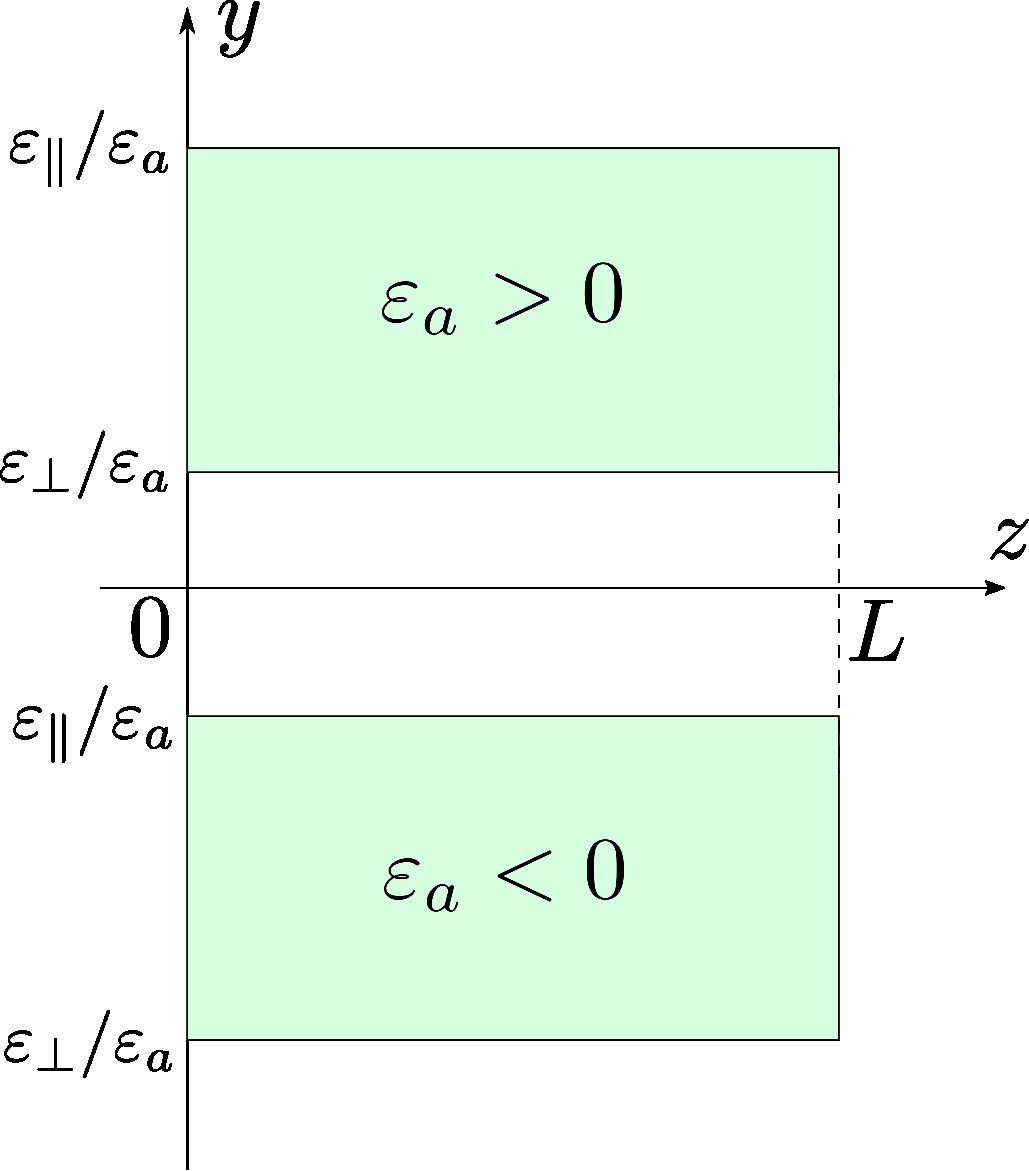
\includegraphics[width=0.55\textwidth]{Allowed_areas_for_y}
	\caption{Графическая иллюстрация системы неравенств~\eqref{eq:rectangle_1}  и~\eqref{eq:rectangle_2} для случаев $\varepsilon_a > 0$ и $\varepsilon_a < 0$.}
\end{figure}
На Рис.~\ref{pic:Allowed_areas_for_y} изображены области, задаваемые неравенствами~\eqref{pic:Allowed_areas_for_y}.
Таким образом, участок кривой $y(z)$ при $z\in[0,\, L]$ должен находиться внутри соответствующего прямоугольника.
Минимум функционалу могут доставлять и такие профили, у которых существуют точки или целые области, где $y(z) = \ve_\|/\ve_a$ или $y(z) = \ve_\bot/\ve_a$.
Обозначим множество таких точек через $A$, а дополнение $A$ до отрезка $[0,L]$ -- $B$.
Проиллюстрируем эти множества на примере графика зависимости $y(
z)$, приведённого на Рис.~\ref{pic:Sample_profile}.
\begin{figure}\label{pic:Sample_profile}
	\centering
	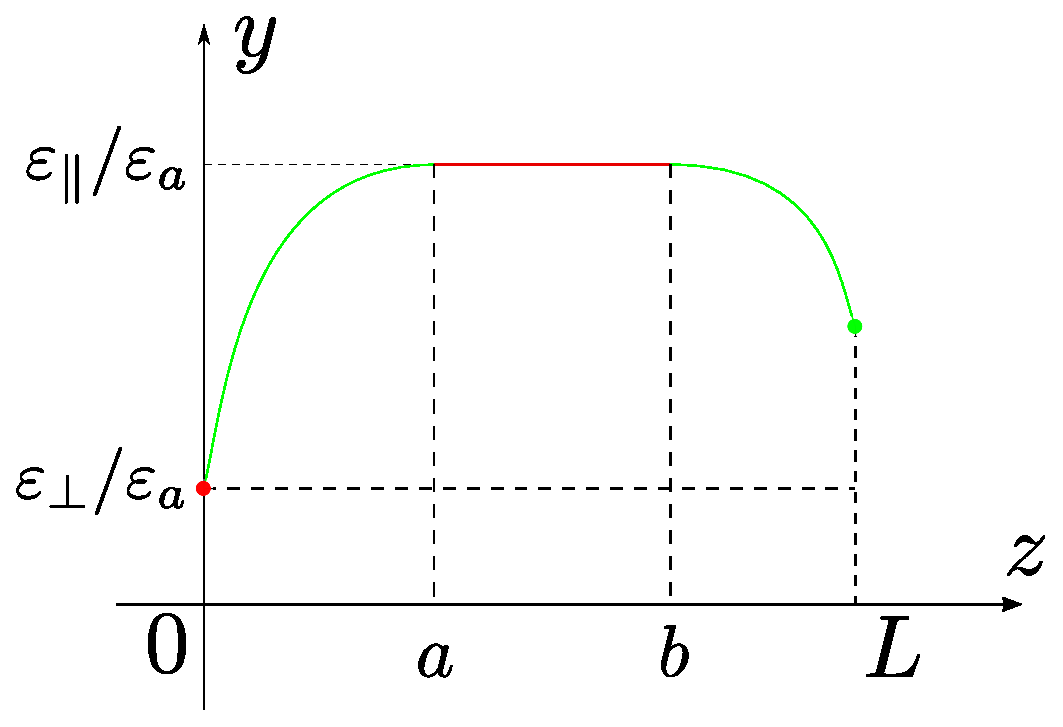
\includegraphics[width=0.7\textwidth]{Sample_profile}
	\caption{График зависимости $y(z)$, иллюстрирующий случай, когда кривая $y(z)$ касается границ ограничивающего прямоугольника.}
\end{figure}
Так, в данном случае $A = \{0\}\cup[a,b]$, $B = (0,a)\cup(b,L]$.
Также важно отметить, что бесконечно малые вариации $\delta y(z)$ произвольны, когда $z\in B$.
В этом случае в условии~\eqref{eq:dF1} может реализоваться только равенство.
Это требование приводит к следующему уравнению Эйлера-Лагранжа:
\begin{align}\label{eq:E-l_y}
&-2yy''+(y')^2 - J^2\left(J_1 - \frac{U}{4\pi\bar{e}}\right)^2 = 0%\\
%&\ve_\bot/\ve_a < y(z) < \ve_\| /\ve_a, \label{cond10}\\
%&0 < z < L.
\end{align}
и граничными условиями
\begin{subequations}
	\begin{align}
		&\bar{e}UJ - 4\pi\bar{e}^2\left( y'(0) + JJ_1 \right) + \ve_a y(0) \frac{W_1}{2} = 0 \label{eq:ch5_boundary1_eq}\\
		-&\bar{e}UJ + 4\pi\bar{e}^2\left( y'(L) + JJ_1 \right) + \ve_a y(L) \frac{W_2}{2} = 0.\label{eq:ch5_boundary2_eq}
	\end{align}
\end{subequations}
Однако при достижении $y(z)$ "верхней" или "нижней" границы прямоугольника~\eqref{eq:rectangle_2}, то есть когда $z\in A$, эти вариации оказываются знакоопределёнными: $\delta y(z) \geq 0$, если $y(z) = \ve_\bot/\ve_a$, и $\delta y(z) \leq 0$ при $y(z) = \ve_\| /\ve_a$.
В этом случае, используя выражение для первой вариации свободной энергии~\eqref{eq:dF_ch5}, для $z\in(0,\ L)\cap A$ вместо уравнения Эйлера-Лагранжа~\eqref{eq:E-l_y} можно записать неравенство
\begin{equation}\label{eq:E-l_ineq}
\left(-2yy''+(y')^2 - J^2\left(J_1 - \frac{U}{4\pi\bar{e}}\right)^2\right)\frac{\delta y}{y} \ge 0.
\end{equation}
Для $z\in \{0, L\}\cap A$ граничные условия также примут форму неравенств:
\begin{subequations}
	\begin{align}
		\left[ -y'(0) - J\left(J_1  - \frac{U}{4\pi\bar{e}}\right) + g_1 y(0) \right]\delta y(0) &\geq 0,\label{eq:boundary1_ch5}\\
		\left[ y'(L) + J\left(J_1  - \frac{U}{4\pi\bar{e}}\right) + g_2 y(L) \right]\delta y(L) &\geq 0,\label{eq:boundary2_ch5}
	\end{align}
\end{subequations}
где
\begin{equation}
g_i = \frac{\ve_a W_i}{8\pi\bar{e}^2},\quad i = 1,2.
\end{equation}
Утверждение.
Если существует некоторый отрезок $[a,\ b] \subset(0,L)$ такой, что множество $[a,b]\cap A$ содержит конечное число элементов, то во всех этих точках $\delta \FF/\delta y = 0$.
Действительно, пусть нашёлся такой отрезок $[a,\ b]$, что существует $z_1$: $z_1\in[a,\ b]\cap A$.
Тогда из непрерывности $\delta \FF/\delta y(z)$ следует, что
\begin{equation}
\frac{\delta \FF}{\delta y(z_1-0)} = \frac{\delta \FF}{\delta y(z_1+0)} = \frac{\delta \FF}{\delta y(z_1)}.
\end{equation}
При этом хотя бы с одной из сторон от $z_1$ $\delta\FF/\delta y(z) = 0$ в силу определения отрезка $[a,\ b]$.
Слеовательно, значение вариации в точке $z_1$ также нулевое.
Утверждение доказано.
	
%Отдельно отметим, что для $z\in\partial A\cap (0,\ L)$ в~\eqref{eq:E-l_ineq} должно выполняться равенство (по непрерывности), а для $z\in\interior{A}$ -- неравенство. 
%Необходимые условия минимума свободной энергии также включают в себя ледующие граничные условия:
%Здесь строгое неравенство соответствует случаю, когда $\{0\}\in A$ или $\{ L \}\in A$, в противном случае имеет место равенство.
При записи условий~\eqref{eq:E-l_ineq}, \eqref{eq:boundary1_ch5} и~\eqref{eq:boundary2_ch5} учтено, что $\ve_a y(z) = \EE(\theta(z)) > 0$.
Отметим, что неравентва~\eqref{eq:E-l_ineq}--\eqref{eq:boundary2_ch5} аналогичны условиям Каруша-Куна-Таккера (см., например,~\cite{Kun-TakkerBook}) для уравнения Эйлера-Лагранжа с граничными условиями.
Таким образом, поиск равновесной ориентационной структуры ЖК-ячейки сводится к достаточно необычной математической задаче: уравнение Эйлера-Лагранжа~\eqref{eq:E-l_y} является интегро-дифференциальным, а также содержит значения искомой функции на границах.
Каждое из граничных условий~\eqref{eq:boundary1_ch5} и~\eqref{eq:boundary2_ch5} -- неравенство и тоже содержит интегральный множитель $J$, зависящий от распределения $\theta(z)$ в объёме ячейки, а также значения $y(0)$ и $y(L)$ в множителе $J_1$.
Наконец, условие, которому должна удовлетворять искомая функция $y(z)$, может быть различным и зависит от того, как распределяются множества $A$ и $B$ на отрезке $[0,\ L]$ для конкретной функции-кандидата. 
%Наконец, если происходит касание границ~\eqref{eq:y_border}, уравнение Эйлера-Лагранжа заменяются неравенством~\eqref{eq:E-l_ineq}.

Достаточное условие минимума свободной энергии может быть получено, если добавить к~\eqref{eq:dF1} требование положительности второй вариации свободной энергии
\begin{equation}
\delta^2\FF[y(z)] > 0,\quad z\in B\cup(\partial A\cap (0,\ L)).
\end{equation}
Во всех остальных точках отрезка $[0,\ L]$ достаточное условие даётся неравенством~\eqref{eq:E-l_ineq}.

Для решения уравнения Эйлера-Лагранжа введём обозначение
\begin{equation}\label{eq:parameter_a}
a = J\left(J_1 - \frac{U}{4\pi\bar{e}}\right).
\end{equation}
Так как выражение $J(J_1 - U/(4\pi\bar{e}))$ не зависит от $z$, получаем параметрическое уравнение
\begin{equation}\label{eq:parametric_EL}
-2yy''+(y')^2 - a^2 = 0.
\end{equation}
Этот параметр также входит в граничные условия~\eqref{eq:boundary1_ch5} и~\eqref{eq:boundary2_ch5}.

Заметим, что если вторая производная  $y''$ равна нулю (а значит, $y(z)$ -- линейная функция), то уравнение~\eqref{eq:parametric_EL} принимает вид
\begin{equation}
(y')^2 - a^2 = 0.
\end{equation}
Семейство линейных функций, являющихся его решениями, может быть описано как
\begin{equation}
y(z) = \pm az + b,
\end{equation}
где $b$ -- произвольная константа.

Далее, путь $y'' \neq 0$.
Введём замену $\tau(y) = y'$.
Тогда справедлива цепочка равенств
\begin{equation}\label{eq:tau_ch5}
y''_{zz} = \tau'_z = \tau'_y y' = \tau'_y\tau.
\end{equation}
Подставляя выражение для $y''$ из~\eqref{eq:tau_ch5} в~\eqref{eq:parametric_EL}, получаем:
\begin{equation}
-2y\tau'_y\tau + \tau^2 - a^2 = 0.
\end{equation}
Разделив переменные и проинтегрировав, запишем
\begin{equation}
\tau^2 - a^2 = cy,
\end{equation}
где $c$ -- произвольная константа.
Учитывая, что $\tau = y'$, проинтегрируем это уравнение:
\begin{equation}
|y'| = \sqrt{cy + a^2} \Rightarrow y = \frac{c}{4}\left( z + b \right)^2- \frac{a^2}{c}.
\end{equation}
Здесь $b$ -- также произвольная константа.

Таким образом, уравнение~\eqref{eq:parametric_EL} имеет три независимых решения
\begin{align}
&y(z) = \pm az + b,\label{eq:linear_solution}\\
&y(z) = \frac{c}{4}\left(z+b\right)^2 - \frac{a^2}{c},\label{eq:parabolic_solution}
\end{align}
где $b$ и $c$ -- произвольные константы.
Выражение~\eqref{eq:parameter_a} является, по своей сути, условием самосогласования на параметр $a$, так как $J$ и $J_1$, в свою очередь, зависят от $a$.
\paragraph{Линейное решение}
Отметим, что из-за требования $y\in C^2[0,\, L]$ кусочно-заданная функция, состоящая из линейных функций~\eqref{eq:linear_solution} решением быть не может.
Подставляя линейное решение~\eqref{eq:linear_solution} в уравнение~\eqref{eq:parametric_EL}, приходим к следующему равенству:
\begin{equation*}
\frac{JU}{4\pi\bar{e}} = 0.
\end{equation*}
Это требование может быть выполнено только в тривиальном случае $U = 0$.
Таким образом, в дальнейшем будем рассатривать только параболическое решение~\eqref{eq:parabolic_solution} с учётом ограничения~\eqref{eq:rectangle_2} на $y(z)$.
Это требование совместно с условиями на границах ячейки~\eqref{eq:boundary1_ch5} и~\eqref{eq:boundary2_ch5}, а также условием самосогласования~\eqref{eq:parameter_a} позволяет определить параметры $a$, $b$ и $c$.
\paragraph{Чисто параболическое решение}
Проверим возможность существования параболического решения $y(z)$ вида~\eqref{eq:parabolic_solution}, для которого было бы выполнено условие $y(z) \in (\ve_\|/\ve_a,\, \ve_\bot/\ve_a) \forall z\in[0,\, L]$.
На языке множеств $A$ и $B$ этот случай соответствует пустому множеству $B$.
Решение должно обладать следующими свойствами:
\begin{itemize}
	\item Абсцисса вершины параболы находится либо вне отрезка $[0,\, L]$, либо её ордината лежит в области возможных значений функции $y(z)$:
	\begin{subequations}
		\begin{empheq}[left = \empheqlbrack]{align}
			&-b \notin [0,\, L]\\
			&\frac{\ve_\bot}{\ve_a}< \frac{-a^2}{c} < \frac{\ve_\|}{\ve_a};
		\end{empheq}
	\end{subequations}
	\item Значения функции $y(z)$ на краях отрезка $[0,\, L]$ также должны находиться в указанном выше интервале:
	\begin{equation}
		\ve_\bot / \ve_a < y(0,\, L) < \ve_\| / \ve_a
	\end{equation}
	\item Должны быть удовлетворены граничные условия~\eqref{eq:ch5_boundary1_eq} и~\eqref{eq:ch5_boundary2_eq};
	\item Должно выполняться условие самосогласования~\eqref{eq:parameter_a}.
\end{itemize}
Подставим исследуемое параболическое решение в граничные условия~\eqref{eq:ch5_boundary1_eq} и~\eqref{eq:ch5_boundary2_eq} и после несложных преобразований получим:
\begin{subequations}
	\begin{align}
		&\left( b + \frac{2a}{c} \right)\left( \frac{g_1}{2}(b - \frac{2a}{c}) - 1 \right) = 0\label{eq:ch5_boundary1_1}\\
		&\left( L + b + \frac{2a}{c} \right)\left( \frac{g_2}{2}(L + b - \frac{2a}{c}) - 1 \right) = 0.\label{eq:ch5_boundary2_1}
	\end{align}
\end{subequations}
Кроме того, вычисляя $J$ и $J_1$ для $y(z)$ заданного вида, запишем условие самосолгасования~\eqref{eq:parameter_a}:
\begin{multline}
a = a \ve_a \left(\ln{\left( \frac{L+b - 2a/c}{b - 2a/c} \times \frac{b+ 2a/c}{L+b+2a/c} \right)} \right)^{-1} \times\\
\times \left( \frac{1}{\ve_a}\ln{ \left( \frac{b - 2a/c}{L + b - 2a/c} \times \frac{b+ 2a/c}{L+b+2a/c} \right)} - \frac{U}{4\pi\bar{e}} \right).
\end{multline}
После преобразований получаем следующее условие:
\begin{equation}\label{eq:ch5_gamma_1}
	L + b - \frac{2a}{c} = \gamma\left( b - \frac{2a}{c} \right).
\end{equation}
Здесь и далее использовано обозначение
\begin{equation}
	\gamma = \exp{\left(\frac{-\ve_a U}{8\pi\bar{e}}\right)}.
\end{equation}
Видно, что условия~\eqref{eq:ch5_boundary1_1} и~\eqref{eq:ch5_boundary2_1} приводят к равенству нулю одного из множителей в каждом условии.
Рассмотрим теперь значения функции $y(z)$ на границах ячейки:
\begin{subequations}
	\begin{align}
		&y(0) = \frac{c}{2}\left( b-\frac{2a}{c} \right)\left( b + \frac{2a}{c} \right)\\
		&y(L) = \frac{c}{2}\left( L + b - \frac{2a}{c} \right)\left( L + b + \frac{2a}{c} \right)
	\end{align}
\end{subequations}
Из того, что они должны быть отличны от нуля, следует, что в условиях~\eqref{eq:ch5_boundary1_1} и~\eqref{eq:ch5_boundary2_1} нулю могут быть равны только вторые множители, что приводит к следующим равенствам:
\begin{align}
&b - 2a/c = 2/g_1\label{eq:ch5_boundary1_2}\\
&L + b - 2a/c = 2/g_2.\label{eq:ch5_boundary2_2}
\end{align}
Видно, что подстановка~\eqref{eq:ch5_boundary1_2} и~\eqref{eq:ch5_boundary2_2} в~\eqref{eq:ch5_gamma_1} даёт
\begin{equation}
g_1 = \gamma g_2.
\end{equation}
Это выражение связывает материальные параметры и не может быть удовлетворено в общем случае.

Рассмотрим решение параболического типа, для которого множество $B$ содержит единственную точку $z_0$.
Как было показано ранее, если эта точка находится на интервале $(0,\, L)$, то уравнение Эйлера-Лагранжа остаётся в силе, а значит, ничего, по сравнению с предыдущим рассмотренным случаем не меняется.
Таким образом, имеет смысл рассмотреть ситуацию, когда $z_0 = 0$ или $z_0 = L$.
Если эта точка находится на левой границе, $z_0 = 0$, то рассмотрим совместно выражение~\eqref{eq:ch5_gamma_1}, возникающее из условия самосогласования, и равенство~\eqref{eq:ch5_boundary2_2}, возникающее из граничного условия~\eqref{eq:ch5_boundary1_2}:
\begin{subequations}
	\begin{align}
		&L+b-\frac{2a}{c} = \frac{2}{g_2}\\
		&L + b - \frac{2a}{c} = \gamma \left(b - \frac{2a}{c}\right).
	\end{align}
\end{subequations}
Выражая $b - 2a/c$ из каждого из условий и приравнивая полученное, запишем:
\begin{equation}
\frac{2}{g_2} - L = \frac{L}{\gamma - 1}.
\end{equation}
Вновь получено равенство, связывающее материальные параметры, а значит, решение такого типа невозможно. Аналогично можно доказать, что случай $z_0 = L$ тоже не реализуется.

Таким образом, для случая чисто параболического решения остаётся рассмотреть ситуацию, когда на обеих границах отрезка $[0,\, L]$.
Введём обозначения
\begin{equation}
	y(0,\, L) = \mu_{0,\, L}.
\end{equation}
Можно записать все условия, которым должно удовлетворять решение:
\begin{subequations}
	\begin{empheq}[left = \empheqlbrace]{align}
		&y(z) = \frac{c}{4}(z + b)^2 - \frac{a^2}{c},\label{eq:ch5_parabolic_system_1}\\
		&y(0) = \mu_0,\label{eq:ch5_parabolic_system_2}\\
		&y(L) = \mu_L,\label{eq:ch5_parabolic_system_3}\\
		&a = J\left(J_1 - \frac{U}{4\pi\bar{e}}\right),\label{eq:ch5_parabolic_system_4}\\
		&-b \notin (0,\, L),\label{eq:ch5_parabolic_system_5}\\
		&\left[ -(y'(0) + a) + g_1 y(0) \right]\delta y(0) \geq 0,\label{eq:ch5_parabolic_system_6}\\
		&\left[ y'(L) + a + g_2 y(L) \right]\delta y(L) \geq 0.\label{eq:ch5_parabolic_system_7}
	\end{empheq}
\end{subequations}
Подстановка зависимости~\eqref{eq:ch5_parabolic_system_1} в~\eqref{eq:ch5_parabolic_system_2}, \eqref{eq:ch5_parabolic_system_3} и~\eqref{eq:ch5_parabolic_system_4} даёт следующую систему уравнений на коэффициенты $a$, $b$ и $c$: \todo{(эта система взята со страницы R-2)}
\begin{subequations}
	\begin{empheq}[left = \empheqlbrace]{align}
		&b = -\frac{L}{2}\left( \frac{\pm \gamma}{\frac{\mu_L}{\mu_0} \pm \gamma} + \frac{1}{1\pm \gamma} \right),\\
		&b - \frac{2a}{c} = \frac{-L}{1 \pm \gamma},\\
		&\frac{c}{4} \cdot \frac{-L}{1 \pm \gamma}\left( b + \frac{2a}{c} \right) = \mu_0.
	\end{empheq}
\end{subequations}
Здесь и далее подразумевается, что во всех выражениях могут стоять одновременно либо только ``верхние'', либо только ``нижние'' знаки.
После несложных алгебраических преобразований удаётся выразить следующие конструкции из коэффициентов, удобные для дальнейшей подстановки:
\begin{subequations}\label{eq:ch5_parabolic_coeff_system}
	\begin{empheq}[left = \empheqlbrace]{align}
		&b = \frac{-L}{2}\left( \frac{\pm \gamma}{\frac{\mu_L}{\mu_0} \pm \gamma} + \frac{1}{1 \pm \gamma}\right),\label{eq:ch5_parabolic_coeff_system_1}\\
		&\frac{2a}{c} = \frac{L}{2}\left( \frac{1}{1 \pm \gamma} - \frac{\pm \gamma}{\frac{\mu_L}{\mu_0} \pm \gamma} \right),\label{eq:ch5_parabolic_coeff_system_2}\\
		&\frac{c}{4} = \frac{\mu_0 \left(1 \pm \gamma\right)\left( \frac{\mu_L}{\mu_0} \pm \gamma \right)}{\pm \gamma L^2}.\label{eq:ch5_parabolic_coeff_system_3}
	\end{empheq}
\end{subequations}
Граничные условия~\eqref{eq:ch5_parabolic_system_6} и~\eqref{eq:ch5_parabolic_system_7} после подстановки в них выражений для коэффициентов~\eqref{eq:ch5_parabolic_coeff_system_1} -- \eqref{eq:ch5_parabolic_coeff_system_3} принимают следующий вид:
\begin{subequations}\label{eq:ch5_some_system}
	\begin{empheq}[left = \empheqlbrace]{align}
		&\mu_0\left( g_1 + \frac{2(1 \pm \gamma)}{L} \right) \delta y(0) \geq 0,\label{eq:ch5_some_system_a}\\
		&\mu_L \left( g_2 + \frac{2(1 \pm \gamma^{-1})}{L} \right) \delta y(L) \geq 0.\label{eq:ch5_some_system_b}
	\end{empheq}
\end{subequations}
\todo{АО: надо придумать, как здесь заменить $\delta y(0,\, L)$ на единицу в некоторой степени.}
Для того, чтобы анализа полученные неравенства, необходимо выбрать знаки $\ve_a$ и $U$.
Произведём расчёт для случая $\ve_a > 0$, $U > 0$.
Заметим, что в этом случае выполнены следующие неравества:
\begin{subequations}
	\begin{align}
		&\mu_{0,L} > 0,\label{eq:ch5_conseq_from_positive_ea_U_1}\\
		&0 < \gamma \leq 1,\label{eq:ch5_conseq_from_positive_ea_U_2}\\
		&1 \leq \gamma^{-1} < \infty.\label{eq:ch5_conseq_from_positive_ea_U_3}
	\end{align}
\end{subequations}
Учитывая требование~\eqref{eq:ch5_conseq_from_positive_ea_U_2}, неравенство~\eqref{eq:ch5_some_system_a} можно свести к требованию $\delta y(0) > 0$, что соответствует $\mu_0 = \ve_\bot / \ve_a$.
Предположим, что знак при $\gamma$ -- ``верхний''.
Тогда неравенство~\eqref{eq:ch5_some_system_b} принимает вид
\begin{equation}
	\left( g_2 + \frac{2(1 + \gamma^{-1})}{L} \right) \delta y(L) \geq 0.
\end{equation}
Выражение в скобках может принимать только положительные значения ($g_i > 0$, так как $\ve_a > 0$).
Таким образом, приходим к требованию $\delta y(L) > 0$, что соответствует $\mu_L = \mu_0 = \ve_\bot / \ve_a$.
Мы получили, что $y(0) = y(L)$, а значит, вершина параболы находится в точке $z = L/2$, а значит, нужно проверить, находится ли ордината вершины на допустимом отрезке.
Выражение для ординаты параболы:
\begin{equation}
y(z)\bigg|_{z = -b} = \frac{-a^2}{c},
\end{equation}
на него наложено следующее ограничение:
\begin{equation}\label{eq:ch5_case1_ineq_system}
\frac{\ve_\bot}{\ve_a} \leq \frac{-a^2}{c} \leq \frac{\ve_\|}{\ve_a}.
\end{equation}
Воспользуемся полученными ранее формулами~\eqref{eq:ch5_parabolic_coeff_system_1}, чтобы выразить $-a^2/c$, и после несложных преобразований получим
\begin{equation}
1 \leq \frac{-(1 - \gamma)^2}{4\gamma}\leq \frac{\ve_\|}{\ve_\bot}.
\end{equation}
Видно, что это условие не выполняется, а значит, решений в случае выбранного при $\gamma$ знака при $\ve_a > 0$ и $U > 0$ нет.

Рассмотрим теперь ``нижний'' знак при $\gamma$.


\paragraph{Решения с участком насыщения}

\todo{Далее -- под переделку, выше -- переписанное.}

Можно заметить, что граничные условия~\eqref{boundary1} и~\eqref{boundary2} могут быть удовлетворены только когда
\begin{align}
&y(0) = \mu_0, \quad\; \mu_0=\ve_\bot/\ve_a \; \text{или} \;  \mu_0=\ve_\|/\ve_a,  \label{y_mu0}\\  
&y(L) = \mu_L, \quad \mu_L=\ve_\bot/\ve_a \; \text{или} \;  \mu_L=\ve_\| /\ve_a, \label{y_muL}
\end{align}
то есть граничные условия могут быть легко проверены путём определения знака выражения, стоящего в квадратных скобках.
\todo{Каких скобках? Непонятно.}
\todo{АО: В статье говорится, что точные выражения для параметров сложные, а здесь нужно привести.}

\todo{Не для иллюстрации, это сама по себе цель.}
Для того, чтобы проиллюстрировать полученные результаты, мы аналитически и численно рассчитали зависимости $y(z)$ и $\theta(z)$.
В дальнейшем ограничимся рассмотрением случая положительно анизотропии диэлектрической проницаемости, $\ve_a > 0$.
Методика поиска равновесной ориентационной структуры ЖК в ячейке путём численной минимизации функционала свободной энергии аналогична таковой, применённой в предыдущих главах.
При этом был использован следующий набор параметров системы: $L = 0.006$~см, $\ve_\bot = 7.2$, $\ve_\|  = 16.2$, $\ve_a = 9$, $\bar{e} = 0.01$~Фр/см.
Было обнаружено, что, в зависимости от значения $g_2 L$, трансформация ориентационной структуры с изменением приложенного напряжения $U$ может происходить по трём различным сценариям.
На Рис.~\ref{ch5:fig1} показана трансформация ориентационной структуры при достаточно небольшой энергии сцепления с правой подложкой $W_\theta^{(2)}$, когда выполнено следующее неравенство:
\begin{equation}\label{ineq_g2L_1}
g_2 L < \frac{2}{\varkappa},
\end{equation}
где $\varkappa = \sqrt{\ve_\| /\ve_a}$.
\begin{figure}[h]
	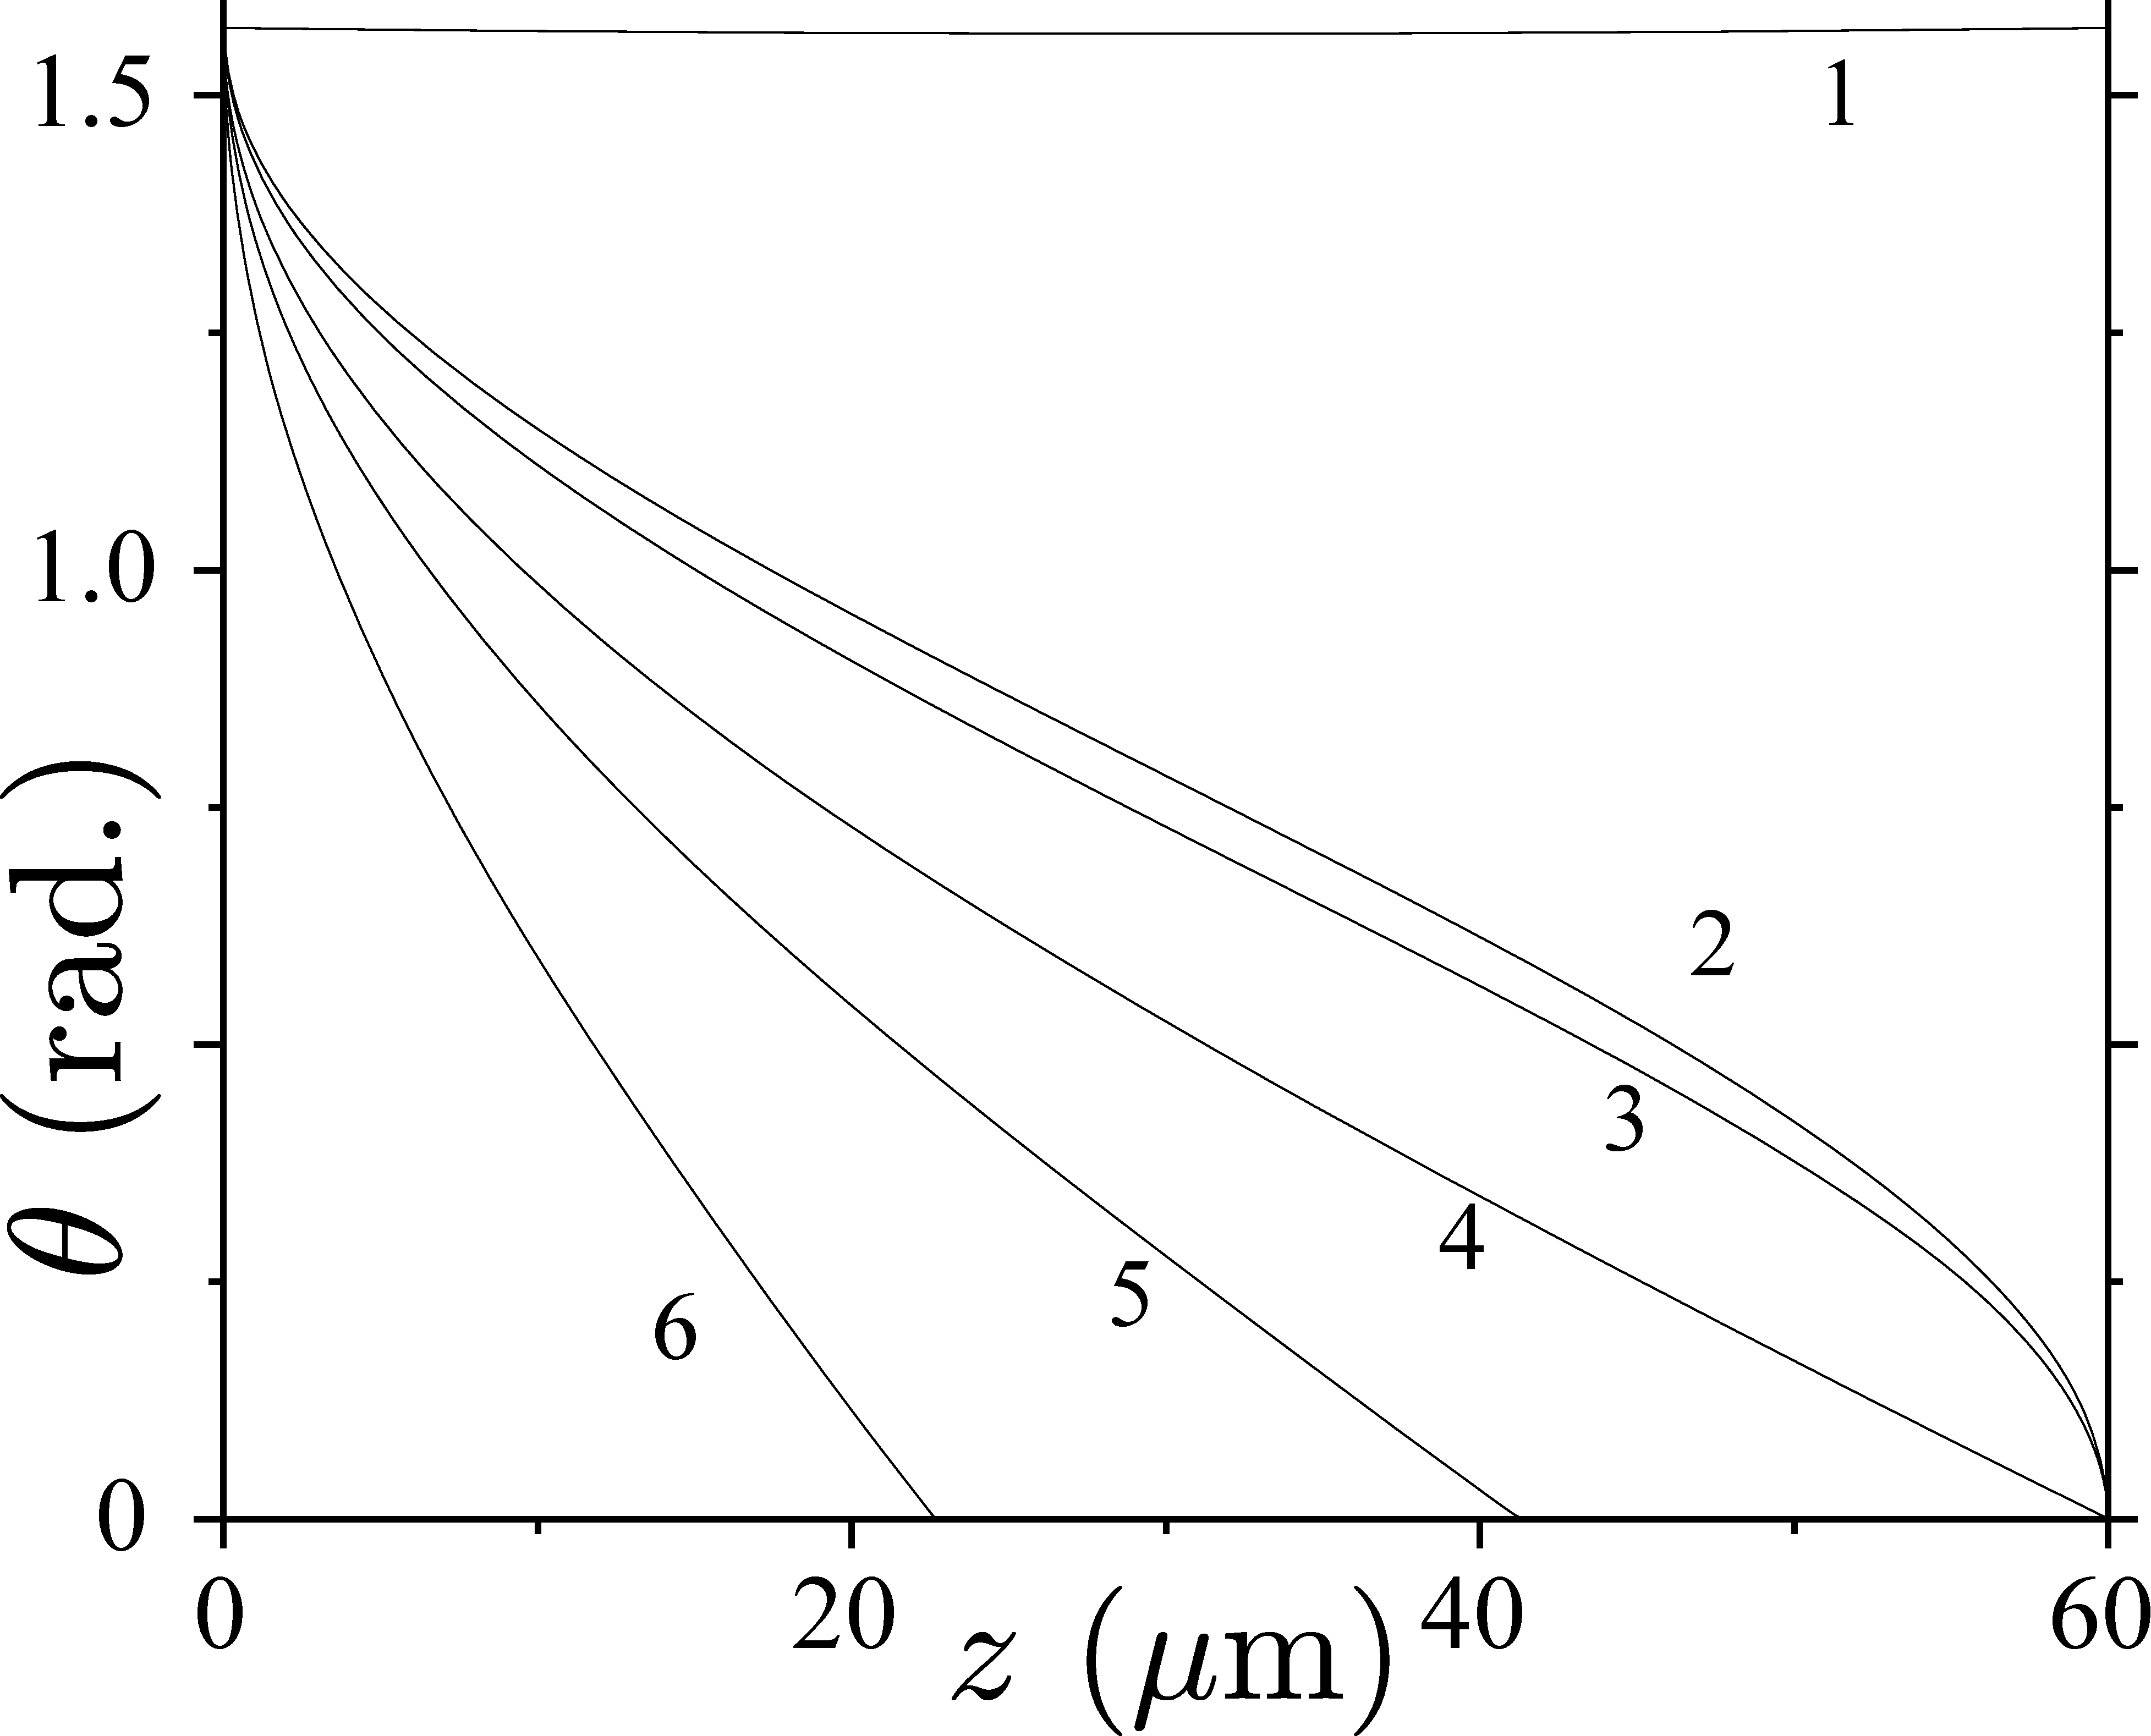
\includegraphics[width=17pc]{Fig1_theta_low_anchoring.eps}\hspace{2pc}%
	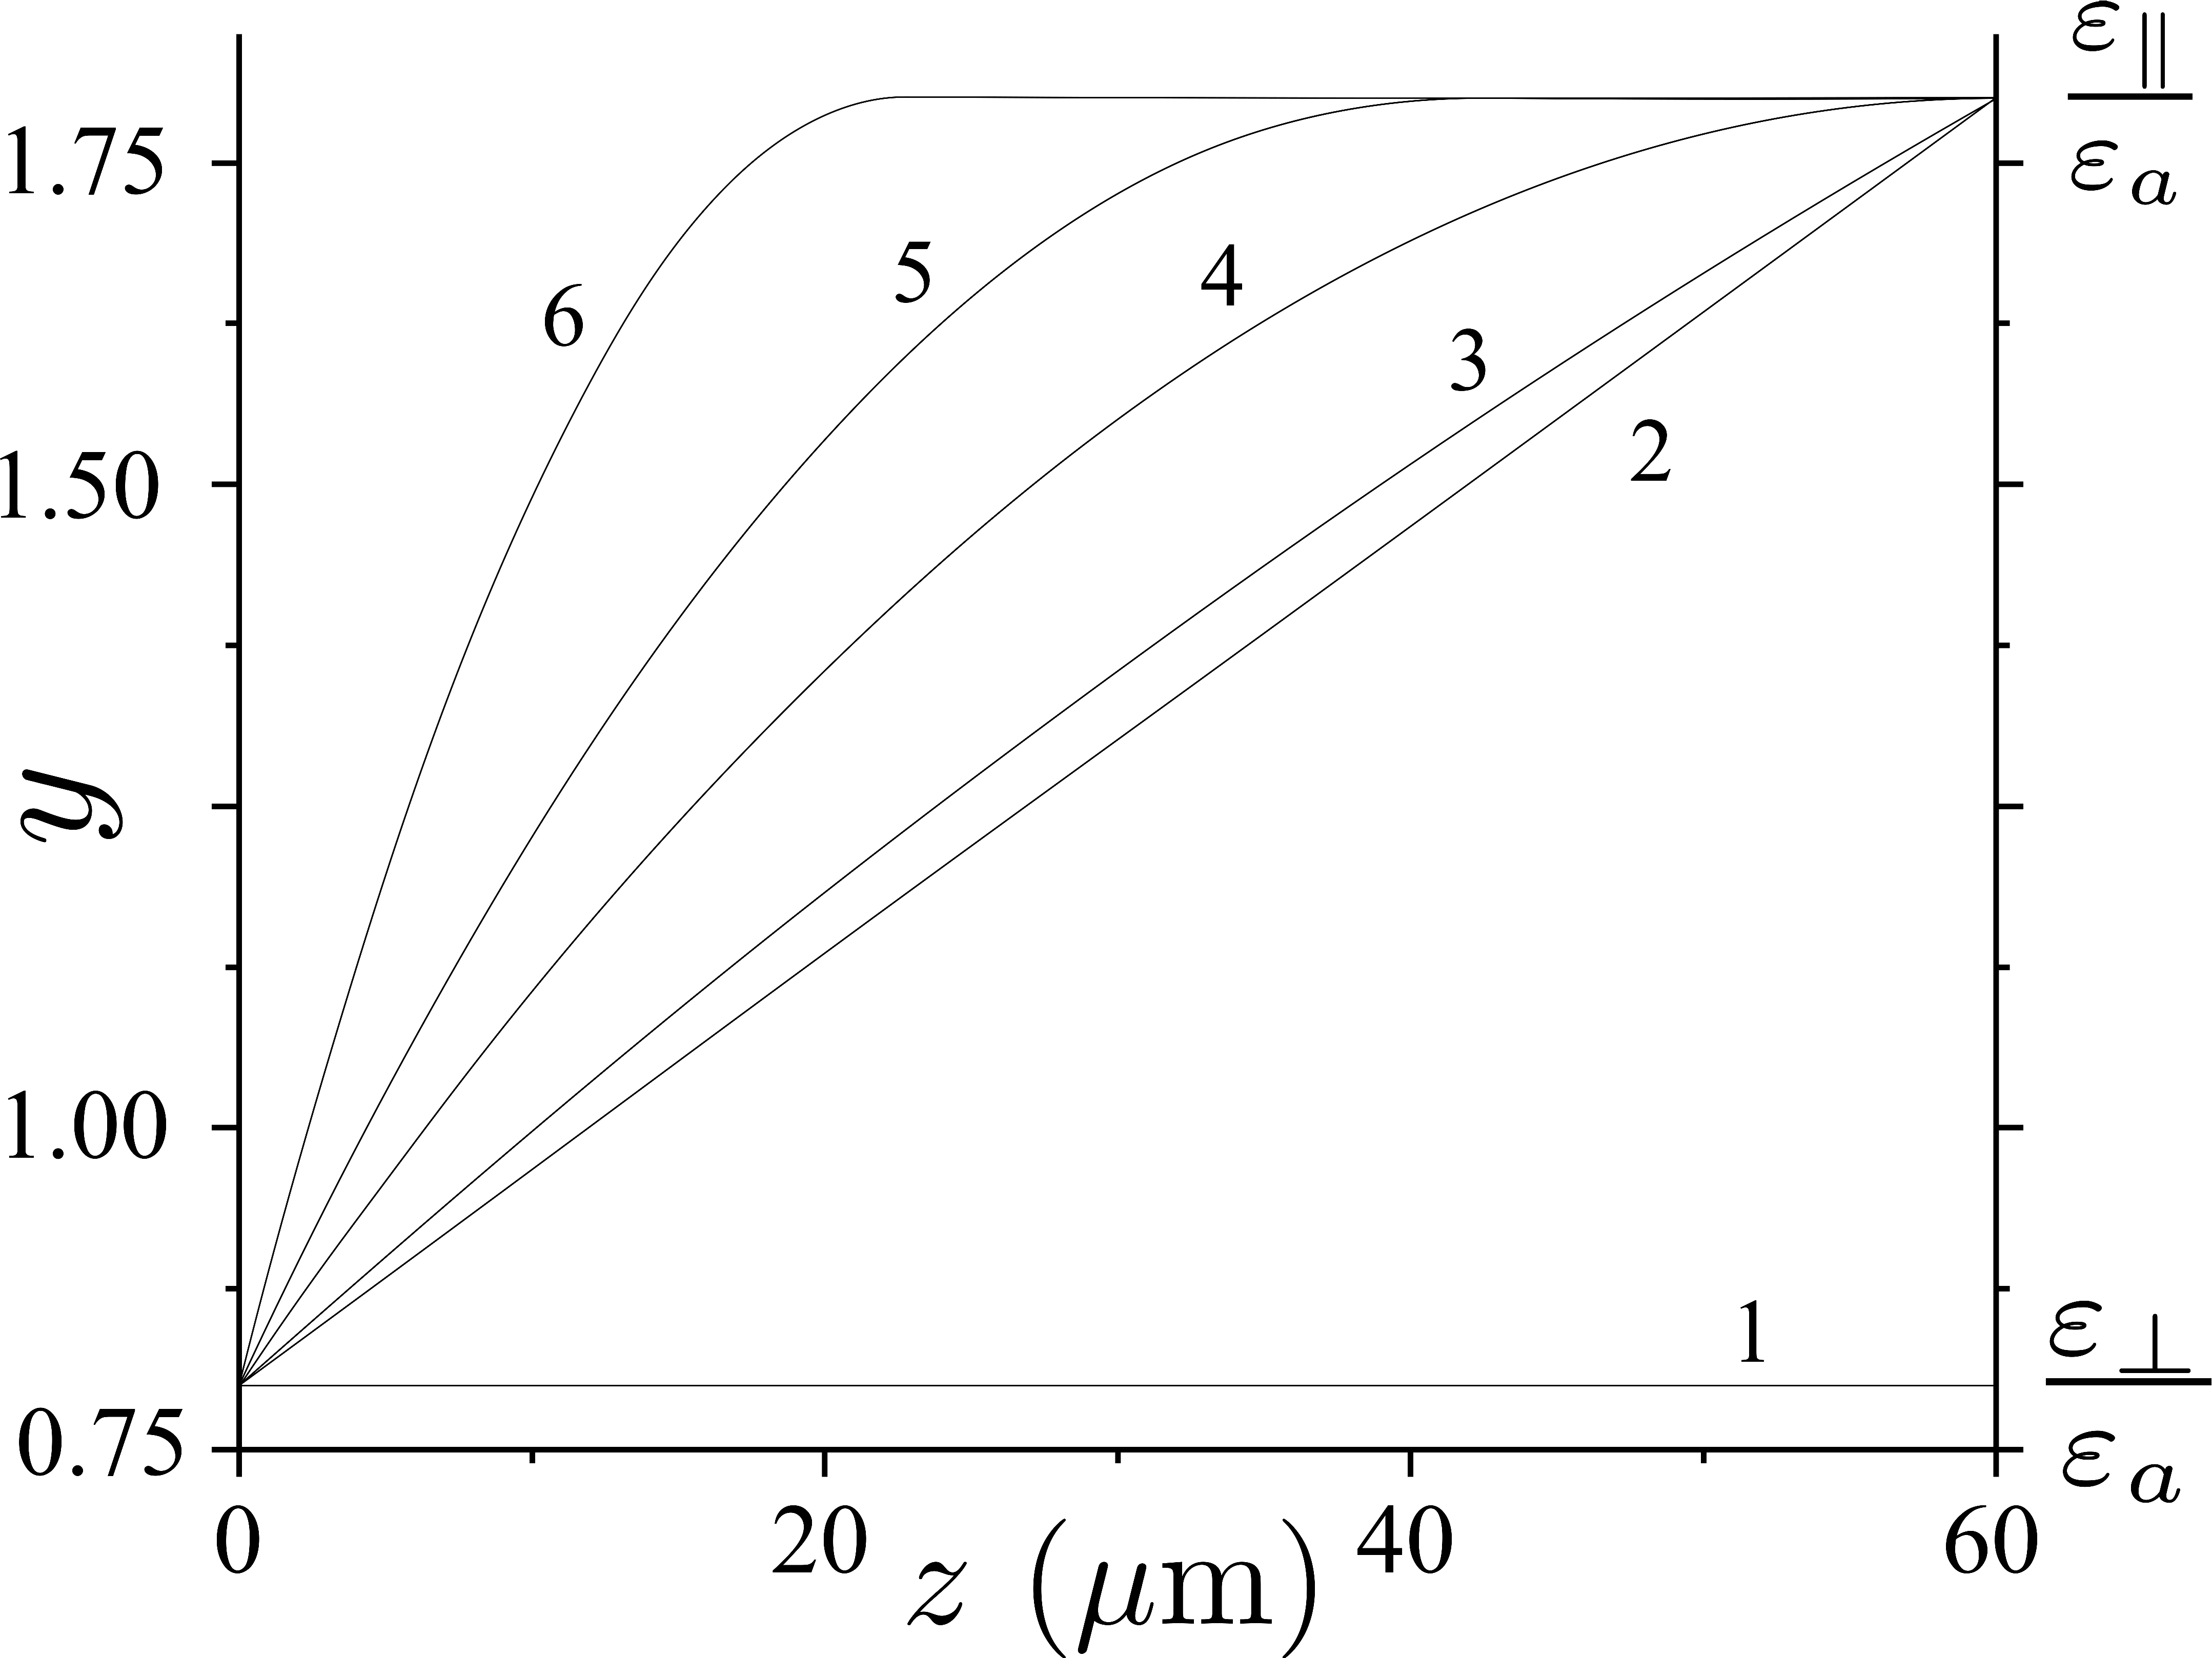
\includegraphics[width=18.8pc]{Fig1_y_low_anchoring.eps}
	\caption{Графики зависимостей $\theta(z)$ (слева) и $y(z)$ (справа), полученные в случае слабого сцепления с правой подложкой, когда выполнено неравенство~\eqref{ineq_g2L_1}.
		Модули сцепления с границами для каждого графика: $W_\theta^{(1)}=0.0025\ \text{эрг}/\text{см}^2$, $W_\theta^{(2)} = 5\times 10^{-4}\ \text{эрг}/\text{см}^2$
		Соответствие линий и приложенного напряжения: 1 -- $U = 0.04$~В, 2 -- $U = 0.05$~В, 3 -- $U = 1.5$~В, 4 -- $U = 4.67$~В, 5 -- $U = 7.5$~В, 6 -- $U = 15$~В.}\label{ch5:fig1}
\end{figure}
Отметим, что кривая $1$ сответствует области малых напряжений $U$, и для неё требование~\eqref{criterion_eU} не выполнено.
Тем не менее, она оказывается близка к зависимости, полученной при помощи численной минимизации полной свободной энергии~\eqref{eq:free-energy}.
Можно также увидеть значительный скачкообразный переход между кривыми $1$ и $2$.
Этот переход происходит при достижении напряжения
\begin{equation}
\widetilde{U}_1 = \frac{8\pi \bar{e}}{\ve_a}\ln{\left( 1 + \frac{g_2 L}{2} \right)}.
\end{equation}
Следует отметить, что для использованных параметров $g_2 L \ll 1$, следовательно, в этом случае $\widetilde{U}_1\simeq W_\theta^{(2)}L/(2\bar{e})$.
С дальнейшим ростом $U$ ориентационная структура меняется без скачков, и при достижении напряжения
\begin{equation}
U_1 = \frac{8\pi \bar{e}}{\ve_a}\ln{\left( \frac{\varkappa + 1}{\varkappa} \right)},
\end{equation}
в объёме ячейки возникает область насыщения, в которой $\theta = 0$, а при увеличении приложенного напряжения эта область увеличивается (см. кривые 5 и 6 на Рис.~\ref{ch5:fig1}).

\todo{``Среднее сцепление''}
В случае, когда константа сцепления с границами удовлетворяет неравенствам
\begin{align}\label{mid_anch}
\frac{2}{\varkappa}< g_2L < \frac{4}{\varkappa - 1},
\end{align}
трансформация ориентационной структуры происходит по другому сценарию, что показано на Рис.~\ref{ch5:fig2}.
\begin{figure}[h]
	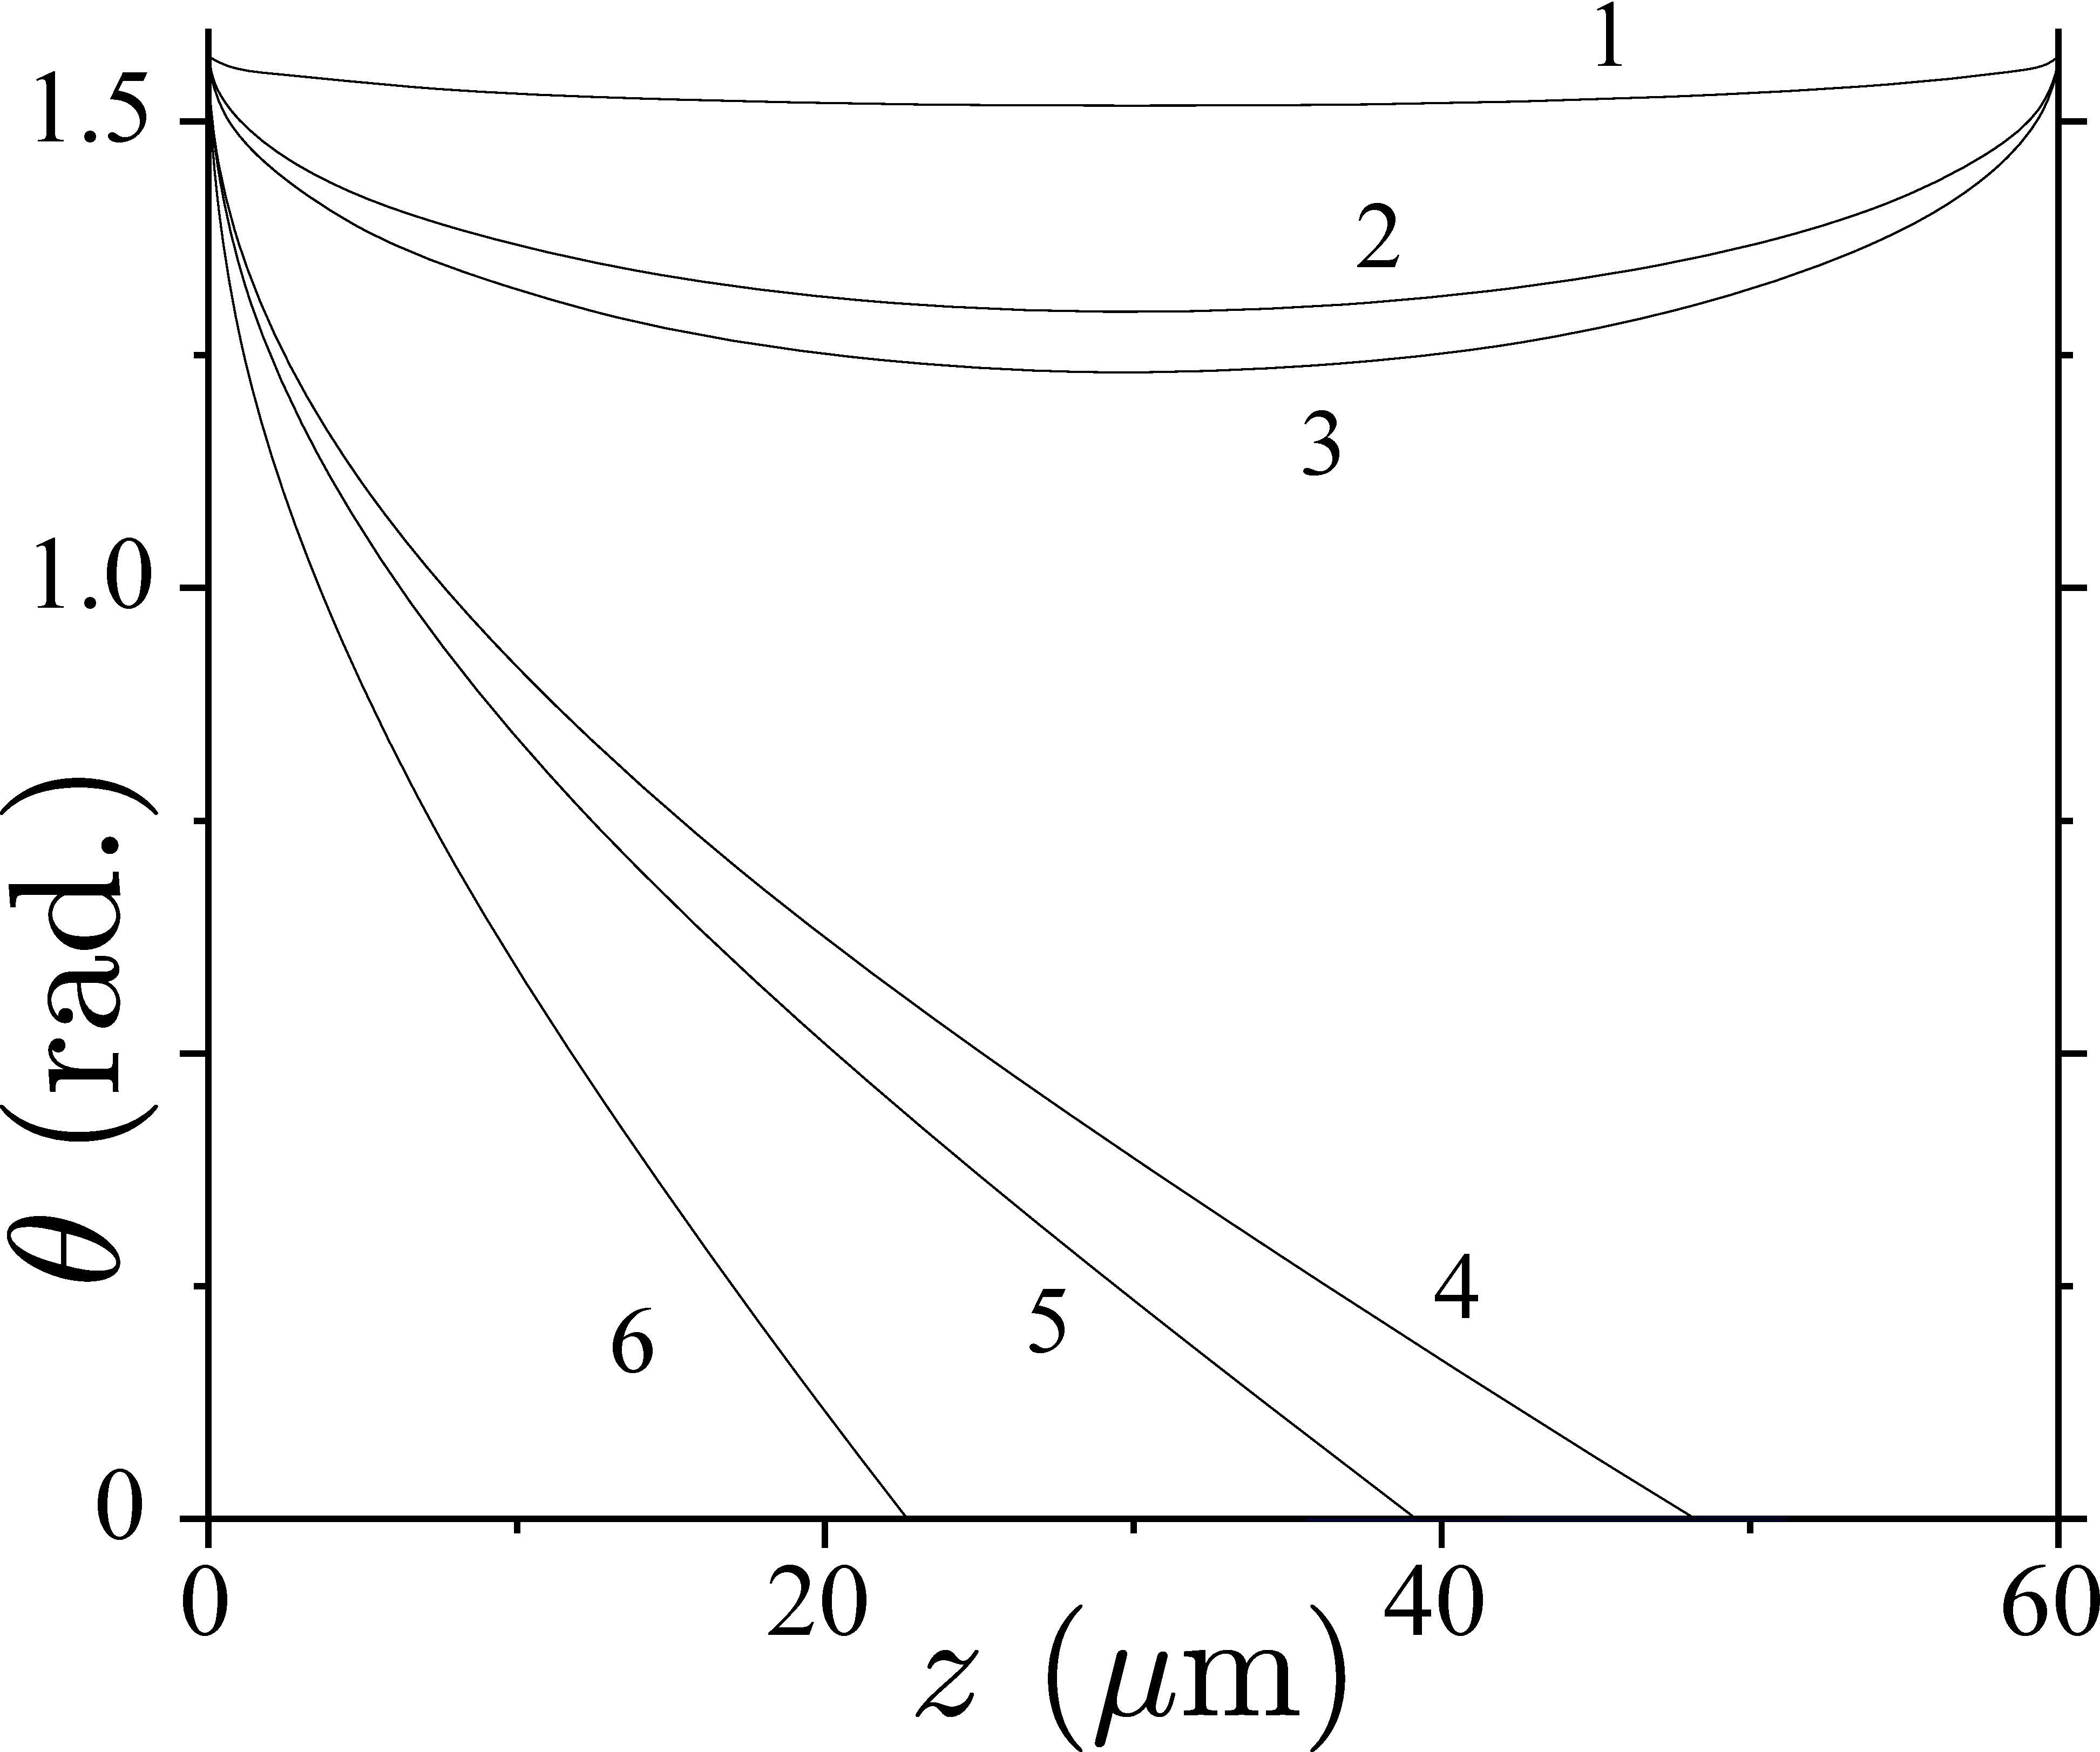
\includegraphics[width=16.9pc]{Fig2_theta_mid_anchoring.eps}\hspace{2pc}%
	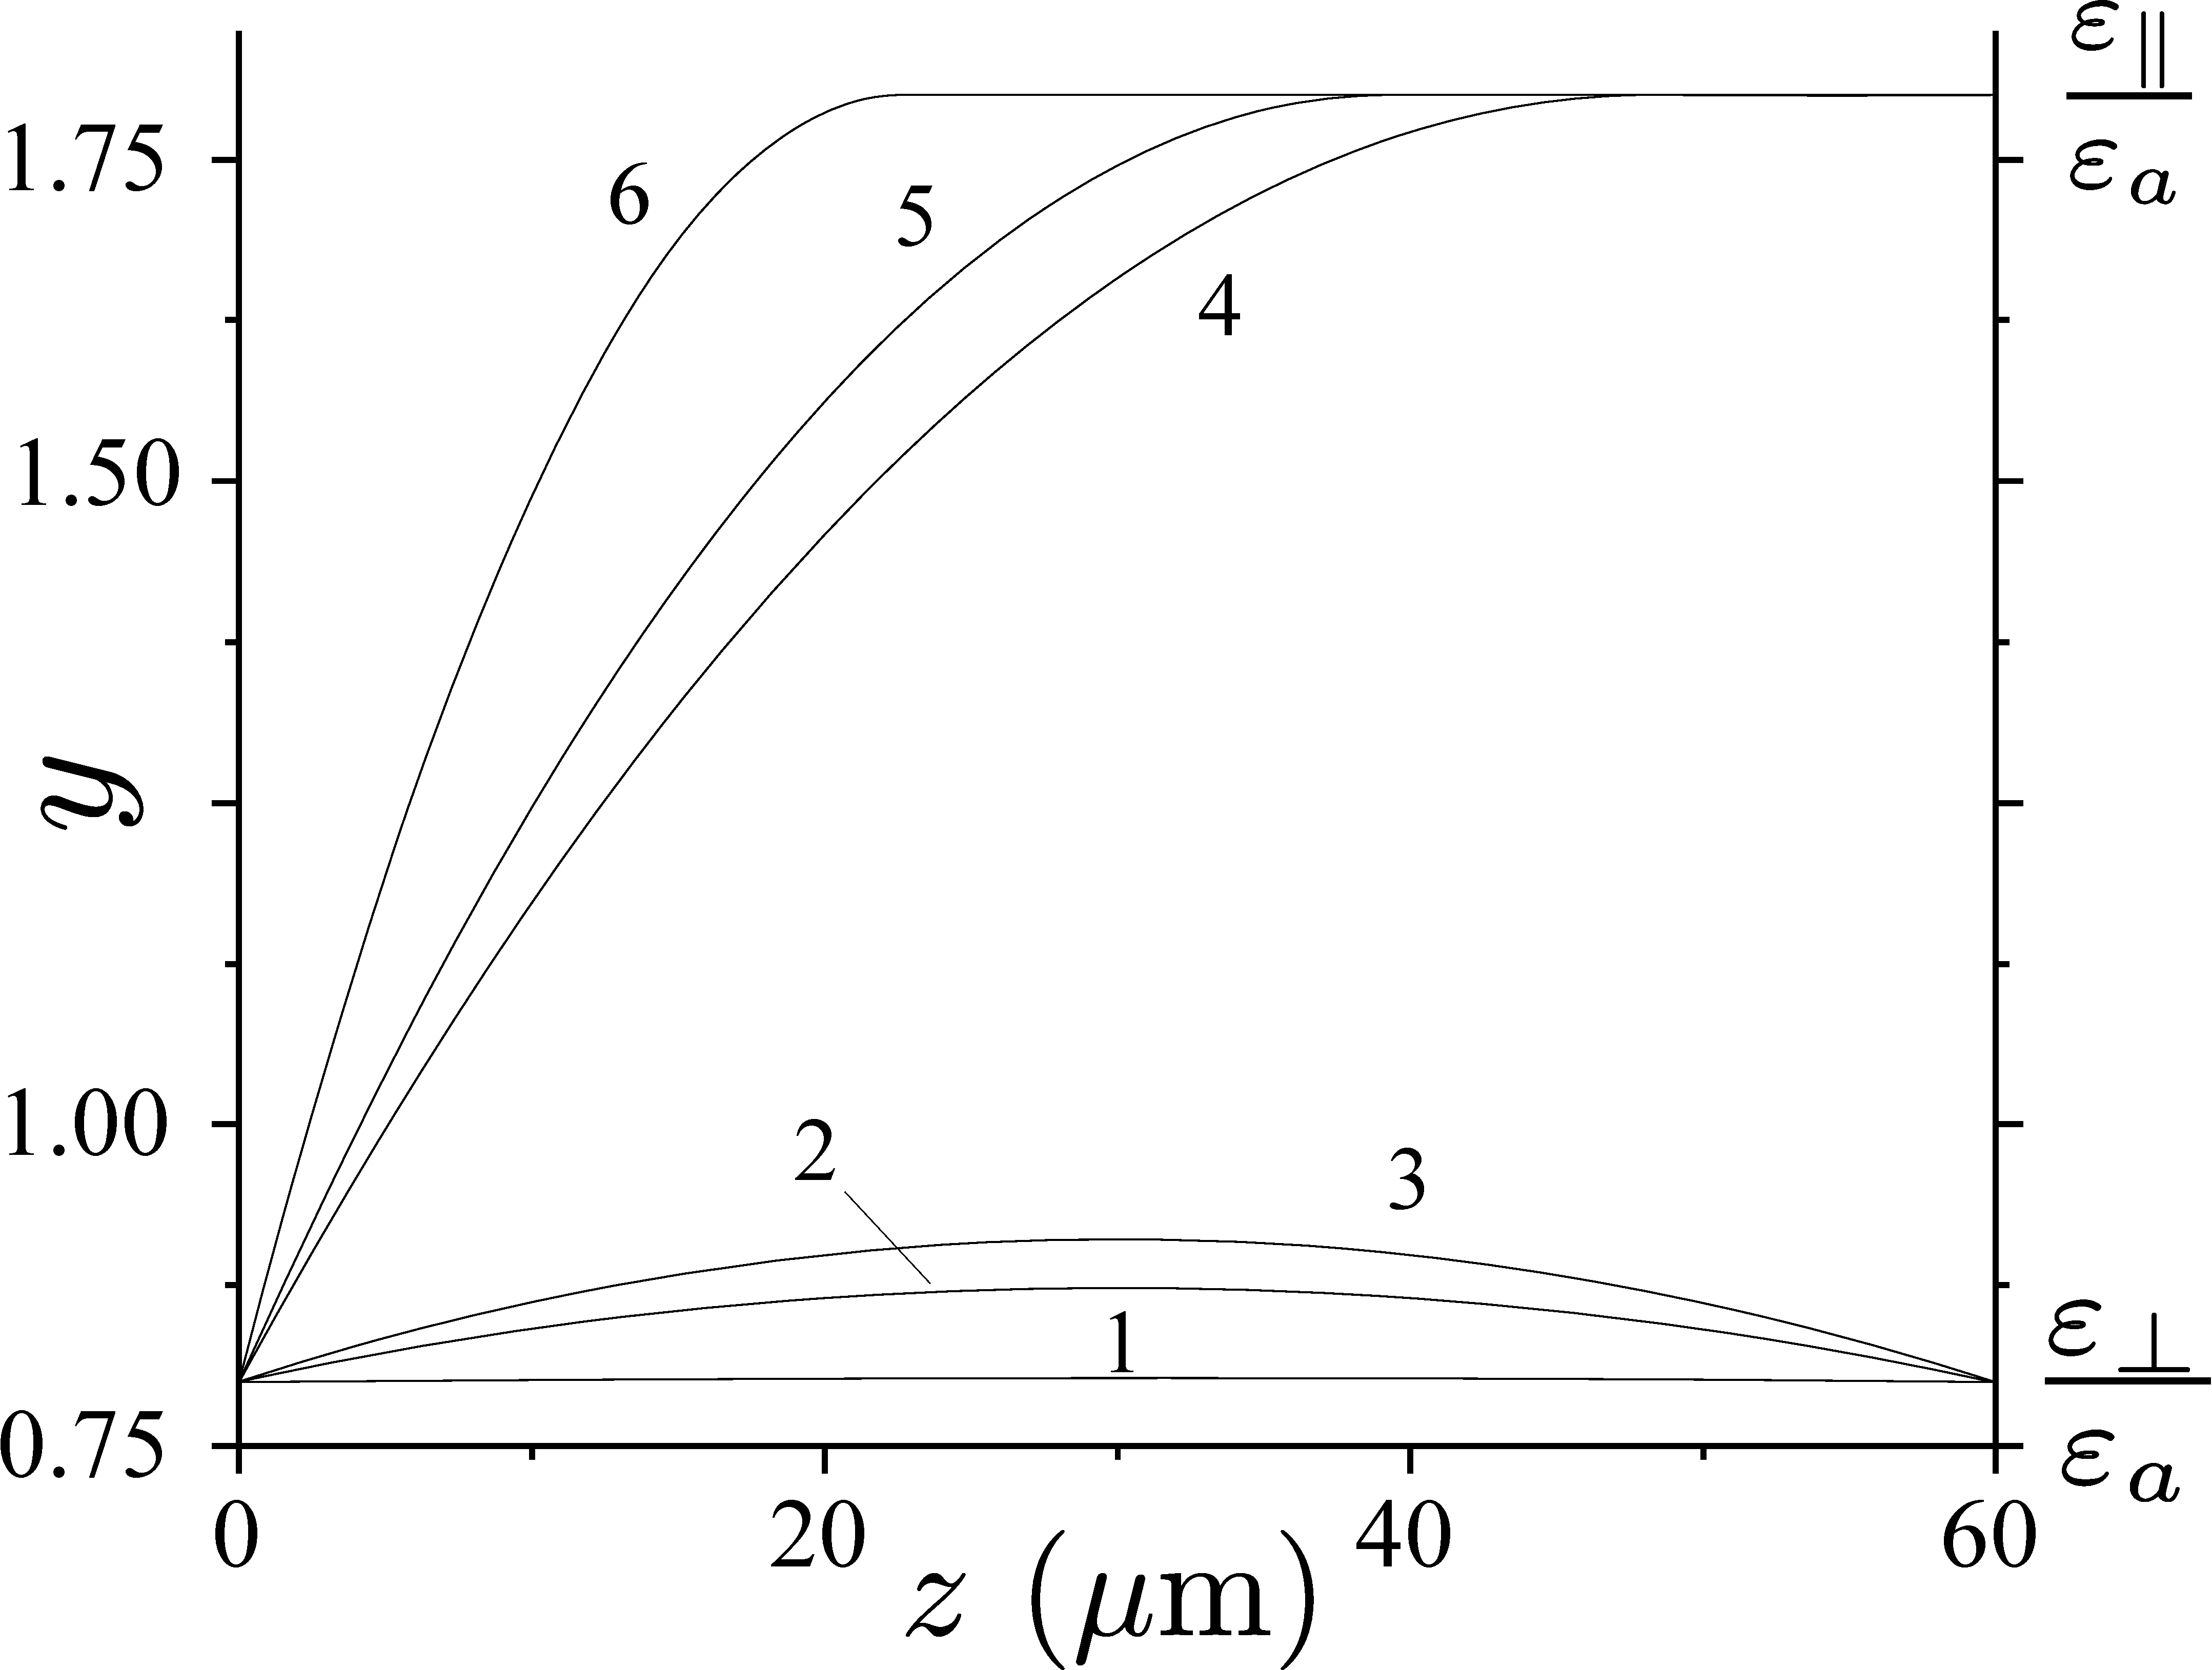
\includegraphics[width=18.9pc]{Fig2_y_mid_anchoring.eps}
	\caption{Графики зависимостей $\theta(z)$ (слева) и $y(z)$ (справа), полученные в случае среднего сцепления с подложкой, когда выполнено неравенство~\eqref{mid_anch}.
		Значения модулей сцепления с подложкой для всех кривых: $W_\theta^{(1)}=0.25\ \text{эрг}/\text{см}^2$, $W_\theta^{(2)} = 0.10\ \text{эрг}/\text{см}^2$.
		Соответствие линий и приложенного напряжения: 1 -- $U = 1$~В, 2 -- $U = 5$~В, 3 -- $U = 6.1$~В, 4 -- $U = 6.2$~В, 5 -- $U = 8$~В, 6 -- $U = 15$~В.}\label{ch5:fig2}
\end{figure}
При этом изменение ориентационной структуры при небольших напряжениях $U$ аналогично происходившим в предыдущем случае, однако когда напряжение достигает значения $\widetilde{U}_1$, происходит скачкообразный переход между кривыми 3 и 4.
Важной особенностью этого случая является то, что область насыщения в объёме ячейки появляется сразу после перехода.
Как и в предыдущем случае, при дальнейшем увеличении напряжения область насыщения в объёме растёт.

\todo{``Сильное зацепление''}

\todo{АО: В описании этого случая ошибка. При отрыве границы она не сразу оказывается насыщенной, и там есть ещё одно характеристическое напряжение}

Наконец, когде энергия сцепления с подложкой удовлетворяет неравенству
\begin{equation}\label{ineq_strong_anch}
g_2L > \frac{4}{\varkappa - 1},
\end{equation}
наблюдается третий сценарий эволюции ориентационной структуры.
\begin{figure}[ht]
	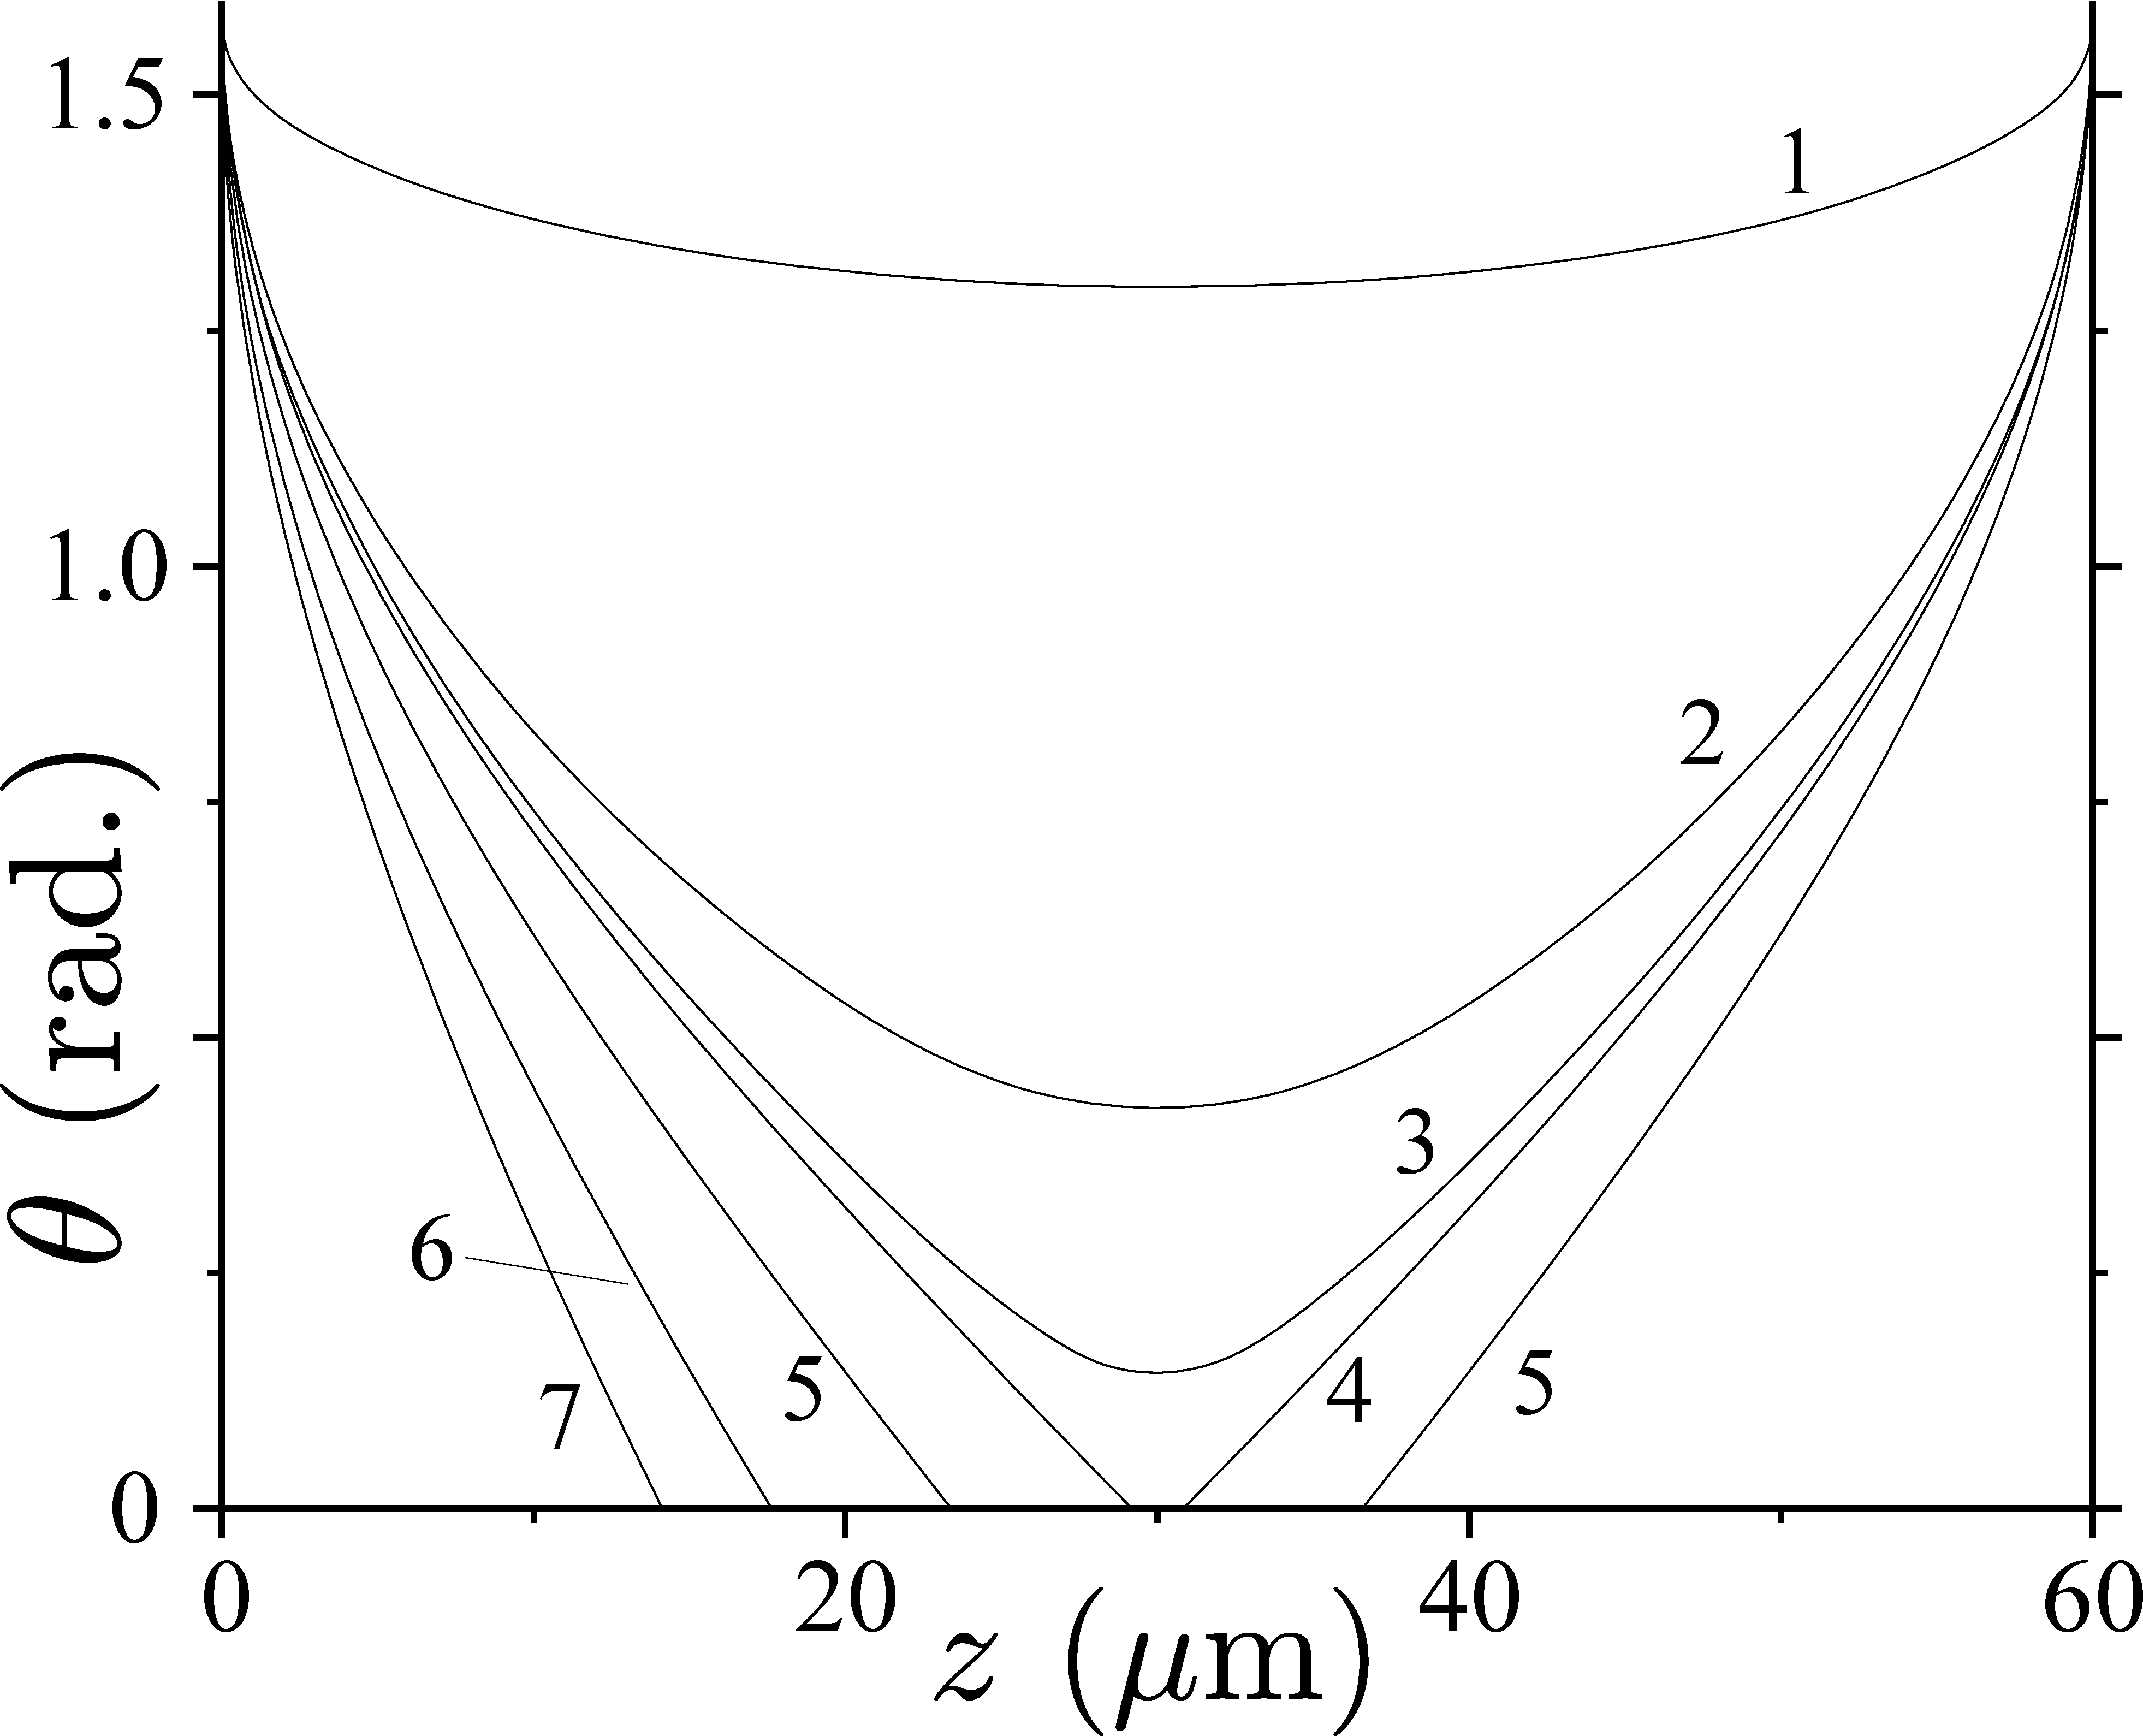
\includegraphics[width=17pc]{Fig3_theta_high_anchoring.eps}\hspace{2pc}%
	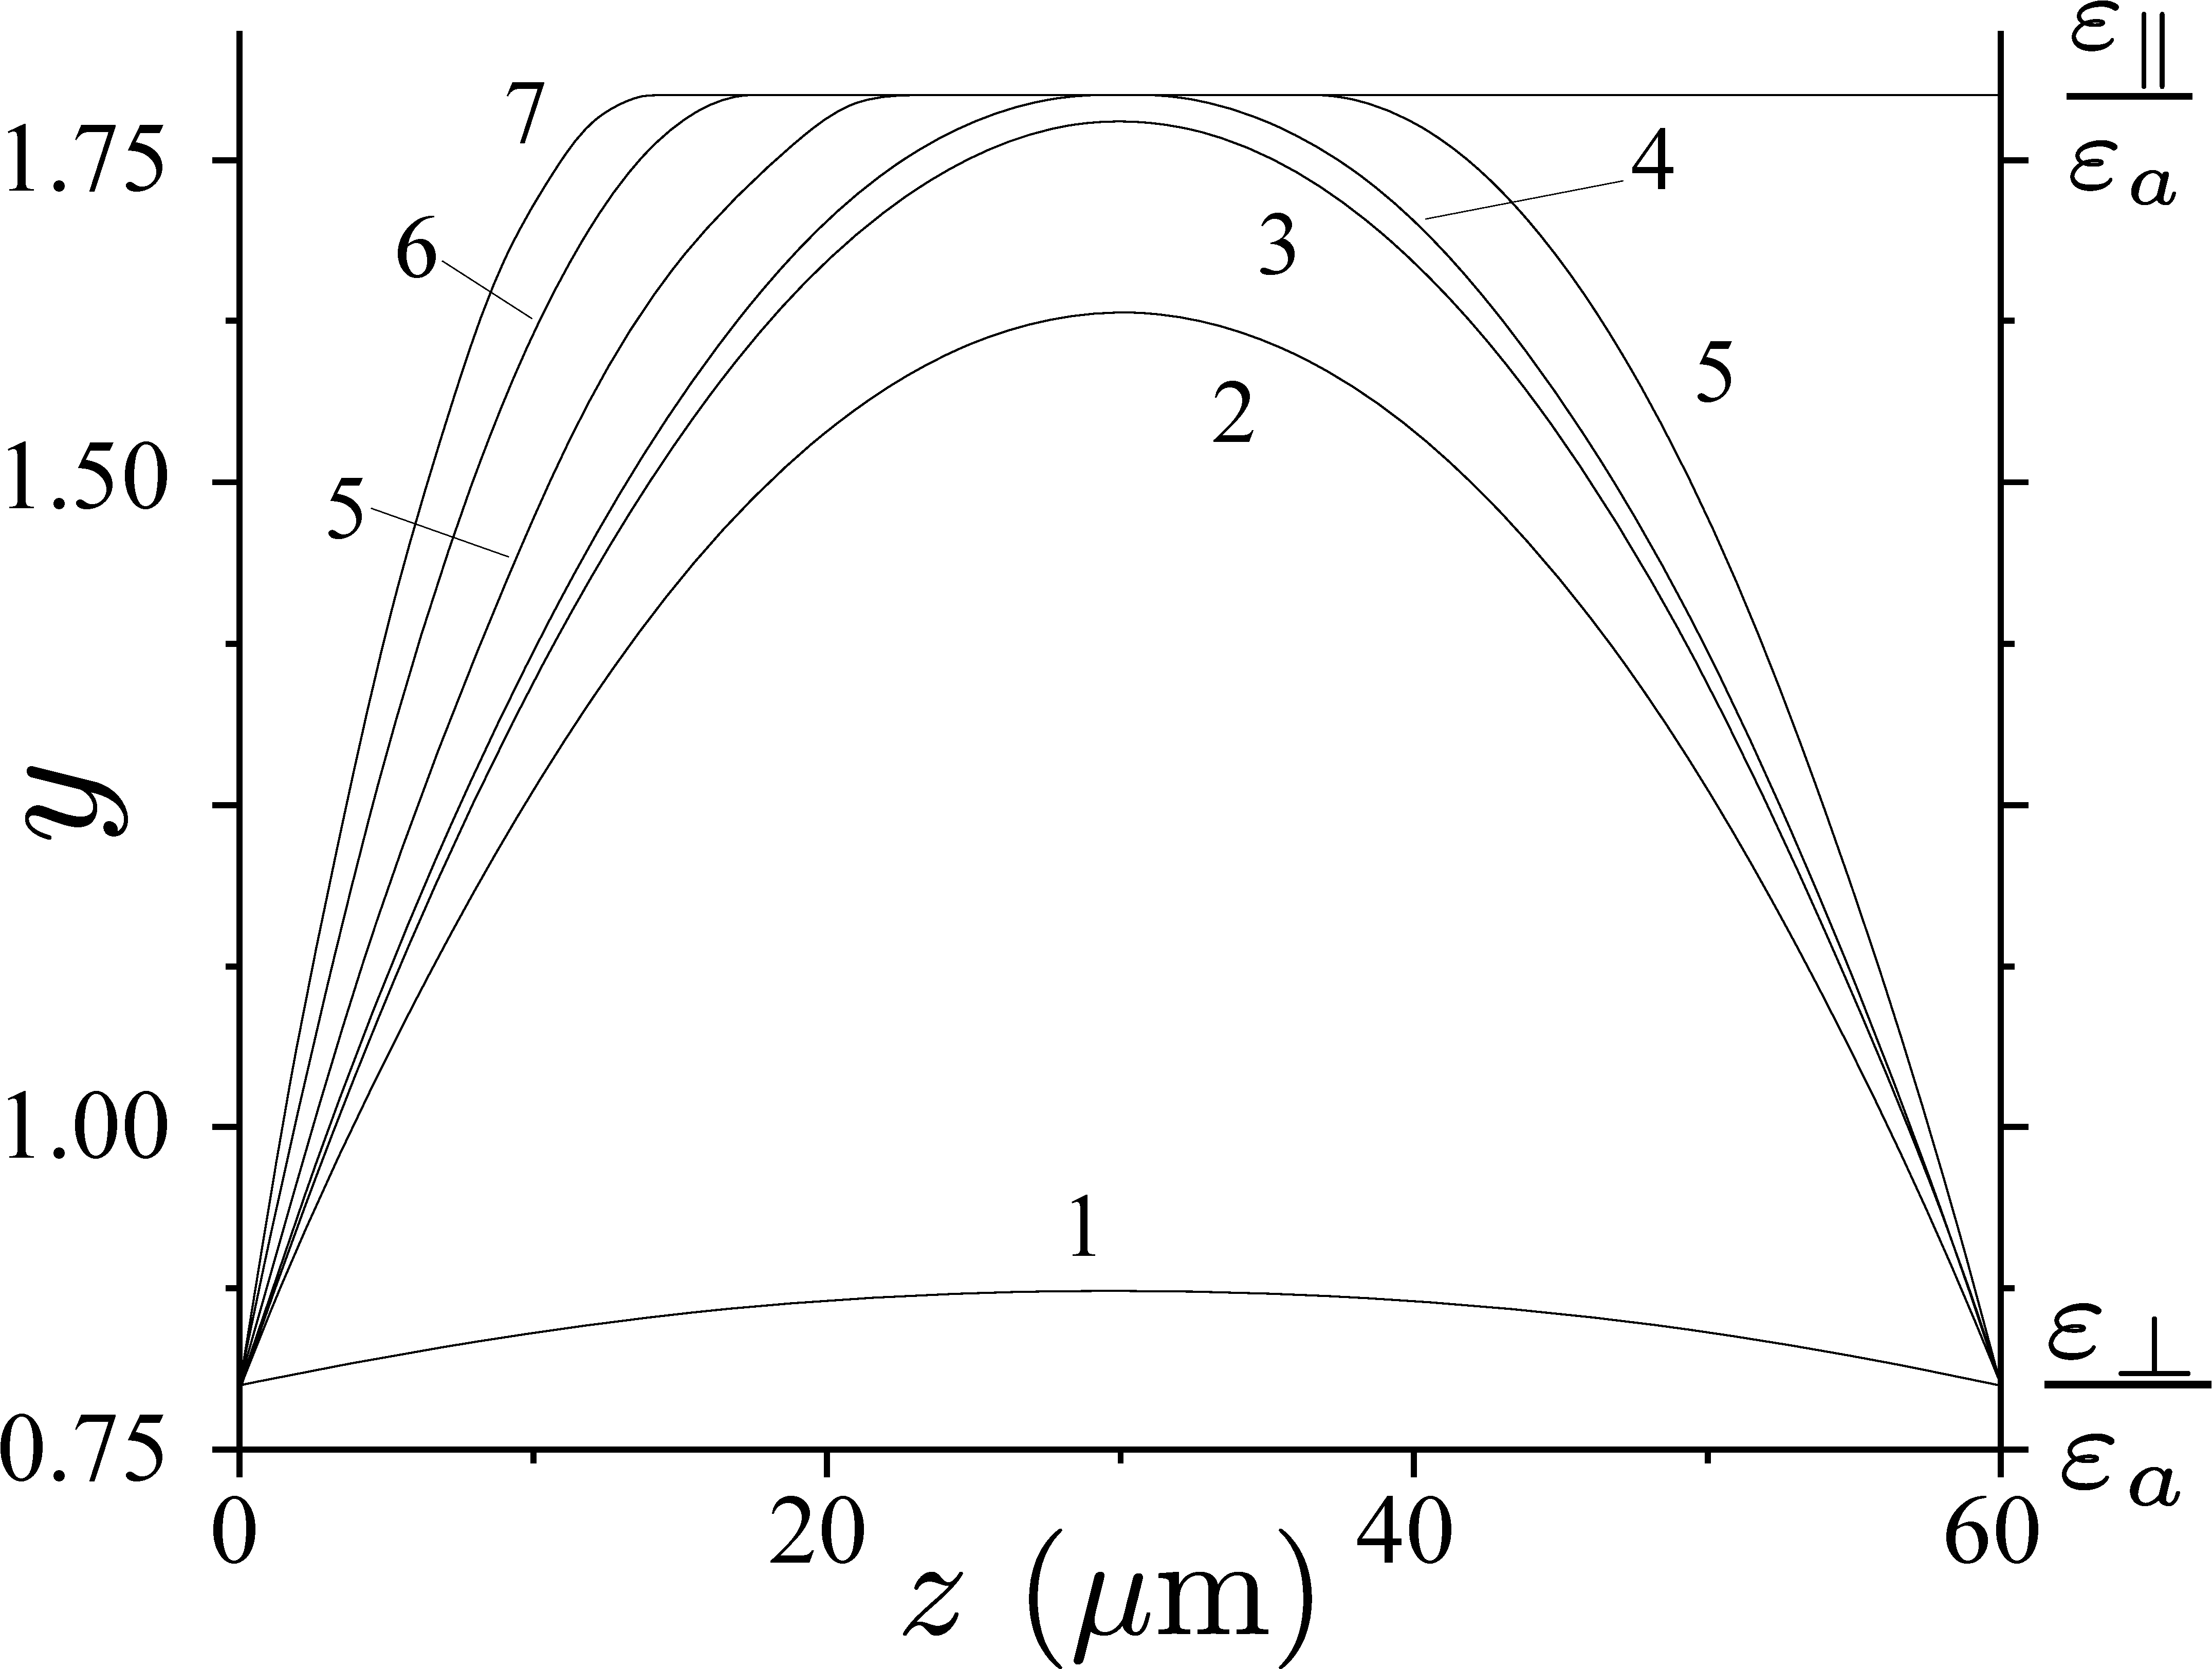
\includegraphics[width=18.9pc]{Fig3_y_high_anchoring.eps}
	\caption{Графики зависимостей $\theta(z)$ (слева) и $y(z)$ (справа), полученные для случая сильного сцепления с подложкой, когда выполнено неравенство~\eqref{ineq_strong_anch}.
		Модули сцепления с подложкой для всех кривых: $W_\theta^{(1)}=1.75\ \text{эрг}/\text{см}^2$, $W_\theta^{(2)} = 0.7\ \text{эрг}/\text{см}^2$.
		Соответствие линий и приложенного напряжения: 1 -- $U = 5$~В, 2 -- $U = 15$~В, 3 -- $U = 16$~В, 4 -- $U = 16.5$~В, 5 -- $U = 19.65$~В, 6 -- $U = 19.75$~В, 7 -- $U = 25$~В.}\label{ch5:fig3}
\end{figure}
Этот сценарий показан на Рис.~\ref{ch5:fig3}.
Опять же, трансформации при малых напряжениях $U$ аналогичны предыдущим случаям.
Однако когда напряжение достигает значения
\begin{equation}
U_2 = \frac{8\pi\bar{e}}{\ve_a}\ln\left( \frac{\varkappa + 1}{\varkappa - 1} \right),
\end{equation} 
в середине ячейки появляется область насыщения (кривые 4 и 5 на Рис.~\ref{ch5:fig3}).
С ростом $U$ эта область продолжает симметрично расширяться от центра ячейки до тех пор, пока напряжение не достигнет значения
\begin{equation}
\widetilde{U}_2 = U_2 + \frac{8\pi \bar{e}}{\ve_a}\left(\frac{g_2L}{2}\cdot\frac{\varkappa}{\varkappa - 1}\cdot \frac{\ve_\bot}{\ve_\parallel} - \frac{2}{\varkappa}\right).
\end{equation}
Когда это происходит, ориентационная структура скачком меняется от описываемой линией 5 на Рис.~\ref{ch5:fig3} до описываемой кривой 6 (при указанном наборе параметров пороговое напряжение составляет $U_2 = 19.68$~В).
Интересно, что если сравнить графики 5 и 6, можно увидеть, что в результате переходе область насыщения расширилась и справа, и слева от центра.
При дальнейшем увеличении $U$ область насыщения также увеличивается (см. линии 6 и 7 на Рис.~\ref{ch5:fig3}).

полученные результаты показывают, что в ячейках с большим усреднённым флексоэлектрическим коэффициентом возможны три сценария эволюции ориентационной структуры с ростом приложенного напряжения.
При этом то, какой сценарий будет реализовываться, зависит от энергии сцепления с одной из границ.
Наши результаты также показали, что в таких ЖК-ячейках возможны разнообразные скачкообразные ориентационные переходы, а также переходы к насыщению.
Такие свойства могут быть использованы при разработке переключателей нового типа.